% Description: Cours de programmation avec le langage Python
% Versions :
%		- v1.0 : avril 2016
%		- v1.1 : octobre 2016 - corrections mineures

%%%
\documentclass[12pt, a4paper]{article}
\usepackage[utf8]{inputenc}
\usepackage[T1]{fontenc}
\usepackage[francais]{babel}
\usepackage[table]{xcolor} %allows to mark some entries in the tables with color
\usepackage{graphicx} % required to import graphic files
\usepackage{float}
\usepackage[font=small]{caption}

\usepackage[left=2cm,right=2cm,top=2cm,bottom=2cm]{geometry} 

% Infos sur le document
\title{Programmation avec Python}
\author{Clément Delgrange}
\date{\today}

% Couleurs utilisées dans le document (code Python essentiellement)
\usepackage{color}
\definecolor{lightgray}{gray}{0.98}
\definecolor{gray}{rgb}{0.6, 0.6, 0.65}
\definecolor{green}{rgb}{0.133, 0.545, 0.133}
\definecolor{blue}{rgb}{0, 0, 1}
\definecolor{red}{rgb}{0.6, 0.1, 0.1}

% Mise en forme des liens hypertextes
\usepackage{hyperref}
\hypersetup{
	colorlinks=true,
	breaklinks=true,
	urlcolor=blue,
	linkcolor=blue,
	pdfborder=000,
	pdftex=true
}

% Mise en forme des codes python
\usepackage{listingsutf8}
\lstset{
	language=python,
	inputencoding=utf8/latin1,
	extendedchars=true,
	keywordstyle=\bfseries\ttfamily\color{blue},
	identifierstyle=\ttfamily,
	commentstyle=\color{gray},
	stringstyle=\ttfamily\color{green},
	showstringspaces=false,
	basicstyle=\footnotesize\ttfamily,
	tabsize=2,
	breaklines=true,
	extendedchars=true,
	xleftmargin=1cm, 
	xrightmargin=1cm,
	backgroundcolor=\color{lightgray},
	literate=%
		{é}{{\'{e}}}1
		{è}{{\`{e}}}1
		{ê}{{\^{e}}}1
		{ë}{{\¨{e}}}1
		{û}{{\^{u}}}1
		{ù}{{\`{u}}}1
		{â}{{\^{a}}}1
		{à}{{\`{a}}}1
		{î}{{\^{i}}}1
		{ô}{{\^{o}}}1
		{ç}{{\c{c}}}1
}

% Définition des entêtes et pieds de page
\usepackage{fancyhdr}
\pagestyle{fancy}
\fancyhf{}
\renewcommand{\headrulewidth}{0pt}
\fancyfoot[L]{Division des enseignements en informatique}
\fancyfoot[C]{-\thepage-}
\fancyfoot[R]{Programmation avec Python}
\renewcommand{\footrulewidth}{0.5pt}

% Personnalisation des titres
\usepackage{titlesec}
\titlespacing{\section}{0em}{4em}{1em}
\titlespacing{\subsection}{0em}{2em}{0em}
\titlespacing{\subsubsection}{0em}{0.5em}{0em}


\setlength{\parskip}{1em}
\renewcommand{\floatpagefraction}{0.3} %default:0.5 allows two big pictures on one page


%%%%%%%%%%%%
%%% Document
%%%%%%%%%%%%
\begin{document}

%%% -------------
%%% Page de titre
%%% -------------
\begin{titlepage}
	\begin{sffamily}
		\begin{flushleft}
			
\includegraphics[scale=0.15]{img/logos/logo_ensg.png}\\[1.5cm]
		\end{flushleft}
		\begin{flushright}
			% pour mettre une image en haut à droite
		\end{flushright}
		
		\vspace{1cm}
		
		\begin{center}
			\hrule
				\vspace{0.5cm}
				{\huge \bfseries Programmation avec Python}
				\vspace{0.7cm}
			\hrule
			
			\vspace{3.5cm}
			
\includegraphics[width=400px]{img/logo_python.png}
			\vspace{5cm}
		
			\large \textit{Division des enseignements en informatique}\\
			\small \textit{v1.1 - octobre 2016}
		\end{center}
	\end{sffamily}
\end{titlepage}


%%% ------------------
%%% Table des matières
%%% ------------------
\addtocontents{toc}{
	\protect\setlength{\parskip}{0pt}
}
\setcounter{tocdepth}{1}
\renewcommand{\partname}{Partie}
\tableofcontents



%%% ------------
%%% Introduction
%%% ------------
\newpage
\part*{Introduction}
Ce cours est une initiation au langage de programmation Python. Il n'est pas nécessaire de déjà connaître ce langage, ni d'avoir des notions avancées en programmation, pour pouvoir l'aborder. Dans la mesure du possible, chaque notion est illustrée d'exemple. Le cours se concentre sur la description du fonctionnement du langage et des syntaxes employées.

Nous reviendrons en premier sur ce qui fait la spécificité de Python : ses caractéristiques, ses usages. Les structures de bases du langage seront ensuite présentées, ce qui nous permettra de construire nos premiers  programmes. Nous aborderons ensuite la modularité en Python pour finir par introduire les bases de la programmation orientée objet dans ce langage. Des notions annexes, mais non moins importantes, comme la documentation, les tests ou la gestion des exceptions s’intercaleront en cours de route.

Des sujets comme la connexion à des bases de données, la réalisation d'interface graphiques ou encore la programmation web ne seront pas abordés dans ce cours. Plus généralement, tout ce qui a trait à l'utilisation de bibliothèques annexes, n'entre pas dans le périmètre de ce cours.

La version 3 de Python est la seule utilisée tout au long du cours.
 
% Pourquoi ce cours
% Quel public
% Pré-requis
% Objectifs
\vspace{2cm}


\begin{footnotesize}
	\begin{minipage}{0.9\textwidth}
		\textbf{\textit{Conventions d'écriture}}
		
		Les conventions d'écriture employées dans ce cours sont les suivantes :
		
		\begin{itemize}
			\item les exemples de codes sont inscrits dans des cadres à fond gris : 
				\begin{lstlisting}
Exemple de code
				\end{lstlisting}

			\item le caractère \lstinline{\%} correspond à un début de ligne dans une console système (il n'est donc pas à recopier).
			\item les caractères \lstinline{>>>} correspondent à des débuts de lignes dans une console Python (ces caractères ne sont pas à recopier).
			\item les lignes ne commençant pas par un caractère spécial sont les résultats de l'exécution d'une commande.
			\item le caractère \lstinline{#} correspond au début d'un commentaire.
		\end{itemize}
	\end{minipage}
\end{footnotesize}




%%% ---------------------
%%% Introduction à Python
%%% ---------------------
\newpage
\part{Introduction à Python}
\chapter{}
Avant d'aborder pleinement la programmation avec le langage Python, nous proposons de nous attarder sur ce qui fait la spécificité du langage Python : son histoire et ses caractéristiques principales en autres. Nous détaillerons ensuite quelques-uns des usages classiques qui peuvent être fait de ce langage. Pour finir cette introduction, nous apprendrons à configurer et utiliser un poste de travail pour pouvoir utiliser le langage Python.



%%% ------------------------------------
\section{L'histoire de Python}
L'histoire de Python débute dans les années 1980 à l'institut national de recherche mathématiques et informatiques des Pays-Bas (CIW) sous l'impulsion de Guido van Rossum. Il y travaille sur le développement d'un nouveau langage de programmation, l'ABC, destiné à être un successeur du BASIC et du PASCAL. 

L'ABC\footnote{Pour plus d'informations sur l'ABC on pourra se reporter à l'ouvrage ABC Programmer's Handbook, Guerts, Meertens, Pemberton, 2005, édition Prentice-Hall} présente la particularité de proposer une invite de commande interactive conservant automatiquement les entrées saisies. L'imbrication du code y est par ailleurs déterminée par l'indentation des lignes, et non pas par des points virgules comme c'est le cas en C ou en Pascal. Mais ce langage présentait plusieurs contraintes de tailles qui empêchèrent sa diffusion à un large public : lecture/écriture de fichiers difficiles, pas de concept de bibliothèque, système d'entrée/sortie peu souple.

Guido van Rossum est ensuite affecté à un projet de mise en place d'un système d'exploitation distribué. Il est chargé de créer un langage de script pour manipuler le système. S'inspirant fortement de l'ABC, dont il essaya de gommer les limitations, il conçut les premières versions d'un langage qu'il appela Python en hommage aux Monty Python qu'il admire.

La première version publique de Python, numérotée 0.9.0, est postée sur un forum en février 1991. Guido von Rossum quitte le CIW en 1995. A cette date Python en est à la version 1.2. Le langage séduit par les possibilités offertes d'ajout de nouveaux objets à partir de fichiers de code Python, de fichiers compilé en C, C++ ou encore Fortran.

Guido von Rossum continue néanmoins de travailler sur le langage Python les cinq années suivantes, en étant soutenu par des fonds de recherche. Python en est alors à la version 1.6.

Puis Guido von Rossum forme l'équipe PythonLabs qui travaillera au sein de différentes structures. Elle permettra à la version 2.0 d'être publiée dès 2000. En 2001 la Python Software Fundation est crée pour supporter le développement de Python et les versions 2.x se poursuivent alors jusqu'à la version 2.7 en 2010. Un système de gestion des compatibilités ascendantes et descendantes entre version est mis en place via un module spécifique, le module \_\_future\_\_.

Une version 3.0  est envisagée pour permettre de rectifier certains défauts du langage (redondance ou obsolescence de méthodes anciennes par exemple) ne pouvant être corrigés sans casser la compatibilité ascendante. Elle verra le jour en décembre 2008. Les développements se poursuivront et Python 3.5 sortira en septembre 2015. 

Depuis la version 2.0.1, Python est distribué par la Python Software Fundation (PSF) sous une licence LGPL (Lesser GNU Public License). Cela signifie que les outils Python peuvent être utilisés sans restriction pour produire des logiciels de tous types, même si ceux-ci sont distribués avec une licence plus restrictive que la GPL. Il est possible de combiner des outils Python à d'autres technologies qui ne seraient pas sous licence GPL pour réaliser des programmes. Le code source de Python lui-même est disponible et modifiable.


%%% ------------------------------------
\section{Caractéristiques du langages}
Avant de commencer à apprendre un langage de programmation, il convient de savoir pourquoi utiliser ce langage plutôt qu'un autre. Dans cette sous-partie, nous nous proposons donc d'explorer les caractéristiques essentielles du langage.

\textbf{Python est portable.} On distingue les langages de programmation compilés des langages interprétés. Les premiers ont pour eux de meilleures performances, mais il nécessitent d'être compilés sur chacune des machines où ils seront exécutés. Les langages interprétés sont généralement moins performants mais peuvent être exécutés directement sur une machine compatible, sans avoir besoin d'être compilé au préalable. Python est un langage interprété compatible avec la plupart des OS du marché (Microsoft Windows, Mas OS, Linux, Android, etc.).

\textbf{Python est un langage orienté objet et fonctionnel.} Python permet de mettre en oeuvre les concepts de l'orienté objet (polymorphisme, héritage, etc.). Mais Python ne s'arrête pas là : c'est aussi un langage de script qui rend possible la programmation fonctionnelle. Il permet ainsi une grande variété d'approches pour résoudre un problème.

\textbf{Python est à typage dynamique fort.} Cela signifie qu'il n'est pas nécessaire de déclarer le type des données que l'on manipule avant de le manipuler. Mais qu'il n'est pour autant pas possible de manipuler ensemble des données dont les types sont incompatibles entre eux.

\textbf{Python est performant.} Python n'est pas un langage interprété "classique". A l'instar du Java, le code source Python est transformé lors de la première exécution en bytecode Python, plus proche du langage machine que le code source, et donc plus rapide lors des exécutions suivantes. Python implémente également un mécanisme de "garbage collector" qui permet de libérer de l'espace mémoire pendant l'exécution du programme et ainsi d'optimiser l'exécution des programmes.

\textbf{Python est associable.} On entend par là que Python peut facilement être combiné à d'autres langages de programmation : il est possible d'appeler une bibliothèque C ou C++ dans un programme Python et inversement pour étendre les fonctionnalités de Python ou améliorer ses performances.

\textbf{Python est facile à lire et à écrire.} En Python, pas de point virgule ou d'accolade pour indiquer la fin d'une instruction ou d'un bloc de code, c'est l'indentation qui fait la structure du programme. Cela rend les programmes écrit en Python très faciles à lire, même pour un débutant en programmation. Par ailleurs, la syntaxe du langage est très simple, notamment comparée à d'autres langages comme le C ou le Java. Un des atouts majeur de Python est ainsi la facilité d'écriture d'un programme.

\textbf{Python est un langage de haut niveau.} Il permet donc d'écrire des programmes en faisant abstraction du matériel utilisé. Il n'y a pas à se soucier de la gestion de la mémoire via l'utilisation de pointeur : les variables sont toujours passées par référence.

\textbf{Python possède une communauté très active.} Python est libre et gratuit, mais cela n'est pas pour autant synonyme d'absence de support. La communauté présente sur les forums internet répond aux question des utilisateurs avec la même efficacité (rapidité, précision) qu'un support commercial. Dans le même ordre d'idées, la documentation est complète et à jour.



%%% ----------------------------------
\section{Python, pour quoi faire ?}
Parfois considéré comme un simple langage de scripts, Python révèle bien d'autres possibilités lorsque l'on s'y intéresse un peu plus. Le champs d'application de Python est très vaste et l'IEEE (Institut des Ingénieurs Electriciens et Electroniciens; organisation dédiée à l'ingénierie et aux sciences appliquées du monde) cite souvent Python comme l'un des cinq langage de programmation les plus utilisés au monde aux côté du Java, C, C++ et C\# (enquêtes se basant sur une dizaine de critères comme les requêtes Google, les commits Github, les offres d'emploi du site Career Builders aux Etats-Unis, etc.).

Le langage Python est par exemple utilisé pour :
\begin{itemize}
	\item Du scripting (adminstration, lecture/manipulation de fichiers, parsing, etc.). C'est la base du langage.
	\item Des scripts en environnements métier. Dans le monde de la géomatique, ArcGIS, QGIS, ERDAS, Autodesk utilisent Python comme langage de script. C'est également le cas de GIMP, Inkscape ou Gedit.
	\begin{center}
		
\includegraphics[width=50px]{img/logo_arcgis.jpeg} \hspace{40px}
		
\includegraphics[width=40px]{img/logo_qgis.jpeg}
	\end{center}
	\item Des calculs scientifiques et du big data. La NASA affirme par exemple utiliser Python comme langage de programmation.
	\begin{center}
		
\includegraphics[width=40px]{img/logo_nasa.jpeg}
	\end{center}
	\item Des applications bureautiques : BitTorrent ou DropBox sont écrit en Python.
	\begin{center}
		
\includegraphics[width=40px]{img/logo_dropbox.jpeg}
	\end{center}
	\item Des extensions. C'est possible par exemple dans ArcGIS ou QGIS.
	\item Des jeux vidéo : Civilization IV ou Battlefield 2 utilisent Python.
	\begin{center}
		
\includegraphics[width=60px]{img/logo_civilization4.jpeg}
	\end{center}
	\item Du web. Python fait parti des langages de programmation utilisés par Google. La plateforme YouTube est écrite en Python. Les groupes de discussion Yahoo l'utilisent également.
	\begin{center}
		
\includegraphics[width=40px]{img/logo_geodjango.jpg} \hspace{35px} 
\includegraphics[width=50px]{img/logo_youtube.jpg}
	\end{center}
	\item Des films d'animation : Pixar utilise Python pour produire ses films d'animation.
	\begin{center}
		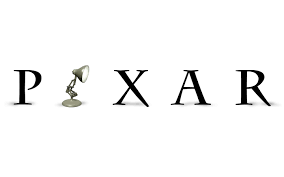
\includegraphics[width=50px]{img/logo_pixar.png}
	\end{center}
	\item Python est également utilisé par des constructeurs de composants informatiques (Intel, Hewlett-Packard, Seagate, IBM) pour tester les performances de leurs nouveaux produits.
\end{itemize}

Pour d'autres exemples d'applications utilisant Python comme langage de programmation, on pourra se reporter à \url{http://www.python.org/about/success/}.

Citons également ici quelques bibliothèques disponibles en Python. Même si l'objet de ce cours ne sera pas de les étudier chacune en détail, il est intéressant d'en connaître quelques unes pour avoir un aperçu des possibilités offertes par le langage :
\begin{itemize}
	\item administration système (gestion de fichier, expression en ligne de commande, etc.) : Sh, Grin, Env, ;
	\item manipulation de réseaux : Scapy, Paramiko, Tornado, Python-oauth2;
	\item interfaces graphiques : Tkinter, WxWindows, PyQt;
	\item développement web : Django, Bottle, CherryPy, Pelican;
	\item intégration de code d'autres langages : Win32, Ctypes;
	\item utilisation de bases de données relationnelles : mysql-python, Psycopg, PyODBC, sqlite3;
	\item mais également NoSQL : PyMongo, Redis, CouchDB;
	\item gestion de données géographiques : Shapely, PySHP, osgeo.ogr, Fiona, ArcPy, PyQGIS, SpatiaLite;
	\item programmation scientifique : Numpy, Scypy ou Matplotlib, Pandas;
	\item manipulation d'images : Pillow, PyOpenGL.
\end{itemize}



%%% ------------------------------
\section{Exécution d'un programme par Python}
\label{sec:execution_programme_python}
Lorsque l'on exécute un code Python, un programme lit notre code et exécute les instructions qu'il contient. Ce programme est appelé un interpréteur Python. Un interpréteur est une sorte de programme qui exécute d'autres programmes.

Lorsque Python est installé sur une machine, un interpréteur Python est systématiquement installé. Cet interpréteur peut prendre des formes diverses (exécutable, jeu de librairies liées dans un programme) et est lui-même implémenté dans un langage de programmation (C, Java ou autre). Sa présence est indispensable pour pouvoir exécuter du code écrit en Python.

L'installation de l'interpréteur Python dépend du système d'exploitation :
\begin{itemize}
	\item Python est généralement installé en standard sur les postes Linux et Mac OS X;
	\item si ce n'est pas le cas, l'utilisateur devra compiler Python à partir des fichiers sources de sa distribution;
	\item sur Windows, l'installation de Python à partir d'un fichier de setup est généralement à faire par l'utilisateur. 
\end{itemize}

Se reporter au site web \url{http://www.python.org} pour le téléchargement de la bonne version de Python.

\underline{Remarque} : certains programmes Windows embarquent leur propre version de Python (ArcGIS ou QGIS par exemple dans le monde de la géomatique). Plusieurs versions de python peuvent alors parfois cohabiter sur le même poste et il convient alors d'être vigilent lors de l'installation de libraires pour être certain qu'elles seront liées à la bonne version de Python.

Pour illustrer le fonctionnement de l'interpréteur Python, nous exécuterons un programme simple se contentant d'afficher \textit{"Hello world !"} dans le flux de sortie. Le fichier .py à exécuter contient uniquement l'instruction suivante :
\begin{lstlisting}
print("Hello world !")
\end{lstlisting}

On peut l'exécuter en faisant \lstinline{python hello_world.py} dans une terminal, en s'étant préalablement placé dans le répertoire contenant le fichier \textit{hello\_world.py}, comme montré figure \ref{fig:hello_world}.

\begin{figure}[H]
	\center 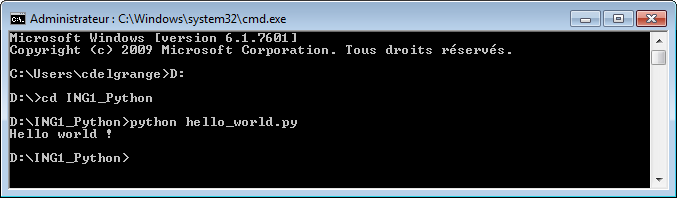
\includegraphics[width=0.8\textwidth]{img/hello_world.png}
	\caption{Hello world en Python}
	\label{fig:hello_world}
\end{figure}

Le code est en réalité compilé en bytecode. Un fichier .pyc est automatiquement créé et c'est ce fichier qui est ensuite interprété par la machine virtuelle Python. La figure \ref{fig:bytecode_execution} représente ce schéma. 

\begin{figure}[H]
	\center 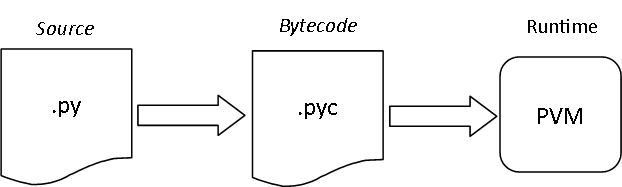
\includegraphics[width=0.5\textwidth]{img/bytecode_execution.png}
	\caption{Fonctionnement de l'interpréteur Python : le code source est traduit en bytecode qui est interprété par la machine vituelle Python (PVM)}
	\label{fig:bytecode_execution}
\end{figure}

Le bytecode n'est pas aussi performant que du C ou C++ compilé puisque la machine virtuelle doit toujours interpréter le bytecode, ce qui est plus couteux en temps que d'exécuter des instructions CPU. Mais, contrairement à un langage interprété classique, Python n'a pas besoin de ré-analyser et re-parser le code source à chaque exécution. La vitesse d'exécution d'un programme Python se situe ainsi quelque part entre celles d'un langage compilé classique et d'un langage interprété classique.



%%% ----------------------------------------
\section{Exécuter un programme en Python}
\subsection{L'invite de commande interactive}
Le premier moyen de faire du Python est d'utiliser l'invite de commande interactive Python (on parle également d'interpréteur intéractif). En supposant que Python ait correctement été installé sur le système, on accède à interpréteur interactif en tapant \lstinline{python} dans une invite de commande.

\begin{figure}[H]
	\center 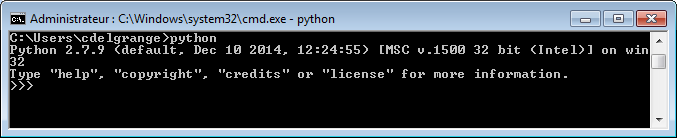
\includegraphics[width=0.8\textwidth]{img/demarrer_session_interactive-1.png}
	\caption{Démarrage classique de l'interpréteur interactif Python}
	\label{demarrer_session-1}
\end{figure}

Lorsque plusieurs versions de Python cohabitent sur le même système, il est possible de préciser quelques options pour appeler une version spécifique. On utilise pour cela la commande \lstinline{py -v} où v est le numéro de la version (note : cette technique n'est plus valable à partir de la version 14.04 d'Ubuntu). Par exemple :

\begin{figure}[H]
	\center 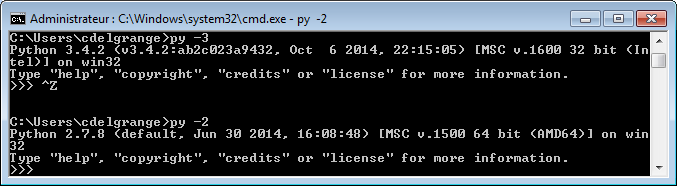
\includegraphics[width=0.8\textwidth]{img/demarrer_session_interactive-2.png}
	\caption{Démarrage d'une version spécificique de l'interpréteur interactif Python}
	\label{demarrer_session-2}
\end{figure}

Sur un poste Windows, on peut également accéder à la ligne de commande Python interactive via le menu démarrer (cf. figure ~\ref{menu_python}).

\begin{figure}[H]
	\center 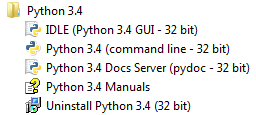
\includegraphics[width=0.4\textwidth]{img/menu_python.png}
	\caption{Menu Python 3.4 du Menu Démarrer de Microsoft Windows 7 lorsque l'installation de Python a été effectuée}
	\label{menu_python}
\end{figure}

Sur un poste Linux où une version Python 2.X cohabiterait avec une version 3.X, la commande python3 permet d'appeler directement la version 3.X de Python, tandis que la commande python lancera généralement la version 2.X (cf figure ~\ref{demarrer_session-3}).

\begin{figure}[H]
	\center 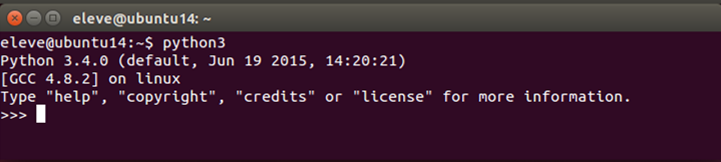
\includegraphics[width=0.8\textwidth]{img/demarrer_session_interactive-3.png}
	\caption{Démarrage d'une version spécifique de l'interpréteur interactif Python sur un poste Linux}
	\label{demarrer_session-3}
\end{figure}

Si la commande \lstinline{python} n'est pas reconnue par votre système, c'est probablement que le chemin d'installation de Python n'est pas présent dans la variable d'environnement PATH. Dans ce cas, il est toujours possible d'appeler explicitement Python comme illustré figure ~\ref{demarrer_session-4}. Cela peut être notamment utile, sur un poste Windows, pour exécuter une version embarquée par un logiciel.
\begin{figure}
	\center 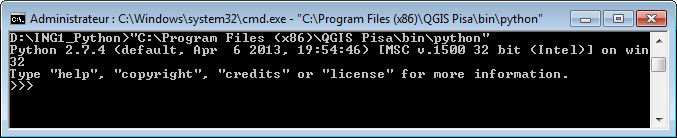
\includegraphics[width=0.8\textwidth]{img/demarrer_session_interactive-4.png}
	\caption{Démarrage de la version de l'interpréteur Python embarquée par QGIS}
	\label{demarrer_session-4}
\end{figure}

La ligne de commande interactive permet d'exécuter des instructions Python. Les instructions sont interprétées et exécutées dès qu'elles ont été saisies. 
\begin{lstlisting}
>>> print("Hello world !")
Hello world !
\end{lstlisting}

La fenêtre garde toutefois en mémoire tout ce qui a déjà été exécuté. Par exemple :
\begin{lstlisting}
>>> x = 3
>>> y = 2
>>> print(x + y)
5
\end{lstlisting}

\underline{Remarque} : pour quitter l'interpréteur Python interactif, on utilise Ctrl-D sur un poste Linux, ou Ctrl-Z + Entrer sur un poste Windows.

Notons qu'il est également possible d'appeler depuis une console l'interpréteur Python pour exécuter un script (c'est ce que nous avons fait dans le premier exemple avec le script hello\_world.py, cf. page ~\pageref{hello_world}). Les schémas vu précédemment pour ouvrir l'interpréteur interactif sont valables également pour exécuter un script :
\begin{itemize}
	\item \lstinline{py -v} pour utiliser un numéro de version spécifique de Python;
	\item \lstinline{python3} pour utiliser Python 3;
	\item \lstinline{C:\chemin_vers_une_version_de_python\python} pour utiliser une version précise.
\end{itemize}

On retiendra également qu'il est possible d'écrire le flux de sortie (les \lstinline{print(...)} dans un fichier texte plutôt que de les afficher dans la console. Pour cela on utilisera la syntaxe :
\begin{lstlisting}
% python script.py > result.txt
\end{lstlisting}

En résumé, l'invite de commande interactive est très utile pour tester des instructions à la volée. En cas de doute sur un extrait de code Python, pour tester une fonction ou un script, c'est l'outil idéal. Mais comme elle ne permet pas de sauvegarder le code, elle se révèle peu efficace pour écrire des programmes en entier. Pour cela, on utilisera plutôt un éditeur de texte. 

\underline{Remarque} : double-clic sur les fichier .py sous Windows
Fichiers .py associés à Python automatiquement sous Windows. Double-cliquer dessus lance interprète de manière transparente. En revanche, si votre script contient uniquement des instructions rapides, quelques \lstinline{print} et se termine, vous n'aurez probablement pas le temps de voir ce qu'il s'est passé. Windows ouvre une invite de commande DOS, appelle l'interprète et exécute le script, affiche les résultats dans l'invite de commande et referme celle-ci une fois les traitements terminés. Pour avoir le temps de visualiser les résultats, on utilisera une astuce qui consiste à ajouter une instruction \lstinline{input()} à la fin du programme (question à l'utilisateur).

Mais si une erreur survient avant la fin de l'exécution, l'instruction \lstinline{input()} ne sera pas lue et l'invite de commande se refermera sans laisser le temps de voir de quelle erreur il s'agit. Bref, sauf à y être contraint pour des besoins de production, on évitera cette méthode pour exécuter un programme Python.


\subsection{IDLE}
IDLE est un outil doté d'une interface graphique et qui permet d'éditer, d'exécuter et de débuger des programmes Python. Il est inclut à l'installation standard de Python et est disponible sur la plupart des plateformes (Windows, Linux, Mac, etc.). IDLE est lui-même écrit en Python (il s'agit en fait uniquement d'un script Python présent dans le répertoire d'installation).

A l'ouverture, on retrouve une console Python, semblable à celle que l'on a utilisé dans le paragraphe précédent (cf. figure ~\ref{idle_console}). Quelques différences notables avec la l'invite de commande Python classique sont tout de même à signaler :
\begin{itemize}
	\item coloration syntaxique des expressions;
	\item auto-complétion avec la touche \textit{Tab};
	\item aide contextuelle lors de l'ouverture d'une parenthèse;
	\item liste de choix lorsque l'on veut utiliser une méthode ou un attribut.
\end{itemize}

\begin{figure}[H]
	\center 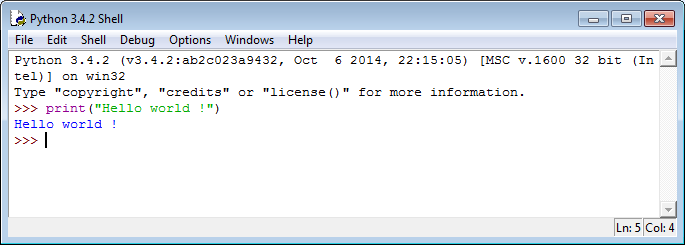
\includegraphics[width=0.7\textwidth]{img/idle_console.png}
	\caption{Console Python de l'interface IDLE}
	\label{idle_console}
\end{figure}

IDLE permet également de parcourir les bibliothèques disponibles (celles installées pour la version de Python utilisée). Enfin, pour créer un programme Python, il faut actionner le menu \textit{File > New File} qui ouvre une seconde fenêtre fonctionnant comme un éditeur de texte avec les même avantages que la console IDLE (coloration, auto-complétion, aide contextuelle, etc. ; cf. figure ~\ref{idle_fenetre}). Le programme peut être exécuté via le menu \textit{Run > Run Module}, ce qui initialise l'interpréteur Python.

\begin{figure}[H]
	\center 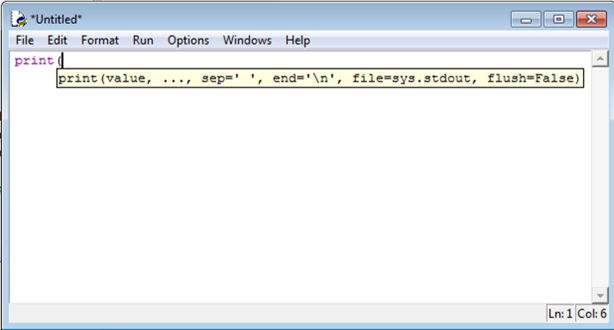
\includegraphics[width=0.5\textwidth]{img/idle_fenetre.png}
	\caption{Fenetre de programme Python de l'interface IDLE}
	\label{idle_fenetre}
\end{figure}

\underline{Remarque} : l'interface et le fonctionnement d'IDLE peuvent être légèrement personnalisés pour rendre son fonctionnement plus agréable. Le lecteur intéressé visitera le menu \textit{Options > Configure IDLE} et testera les différentes options.


\subsection{Environnements de développement intégrés}
Il existe de nombreux environnements de développement permettant d'écrire des programmes en Python. Cette partie se contentera d'en lister quelques uns. Le choix d'un environnement de développement intégré (IDE) pour Python relèvera essentiellement du goût personnel pour un outil plutôt que de critères techniques.

\begin{itemize}
	\item \textbf{PyScripter}\footnote{\url{http://sourceforge.net/projects/pyscripter/}} : environnement de développement léger qui intègre un éditeur de texte, une console Python et un explorateur de solution dans la même fenêtre. Permet de faire du débogage de code.
	\item \textbf{PyCharm}\footnote{\url{http://www.jetbrains.com/pycharm/}} : environnement de développement complet de l'éditeur Jet Brains. Une version gratuite et une version payante comprenant plus de fonctionnalités (intégration de framework web Django, Pyramid, etc. ainsi qu'une interface de gestion de bases de données).
	\item \textbf{Eclipse et PyDev}\footnote{\url{http://www.pydev.org/}} : Eclipse est un environnement de développement prenant en charge de nombreux langages de programmation, dont Python via l'extension PyDev.
\end{itemize}



\subsection{Autres outils utiles}
IPython (Jupyter) / Notebook : possibilité d'intégrer du code Python à du texte et d'exécuter ce code Python pour voir le résultat. Très utile pour l'étudiant pour prendre des notes, sauvegarder des morceaux de code avec les explications qui vont avec.




%%% -------------------
%%% Types et opérations
%%% -------------------
\newpage
\part{Types et opérations}
\chapter{}
Ce chapitre va nous permettre de commencer à utiliser le langage Python. Nous nous limiterons pour commencer à des opérations basiques comme des opérations mathématiques ou des manipulations de chaînes de caractères. Plus précisément, nous nous limiterons dans ce chapitre aux opérations sur des types de base définis dans le langage.

Avant cela, nous définirons ce que sont une variable et un type en informatique. Nous introduirons un concept important en Python, le typage dynamique, et montrerons comment sont gérées données dans ce langage.

%instruction, blocs d'instructions
%fonction / méthode


%%% ---------------------------------------
\section{Variables et types en Python}
\label{sec:variables}

%%%
\subsection{Généralités}
La programmation consiste essentiellement à manipuler des données. Ces données de natures diverses sont stockées sous forme binaire dans la mémoire de l'ordinateur. Pour y accéder, un programme définit des \textbf{variables}.

Nous définirons ainsi une variable comme l'association d'un nom et d'une valeur. Le nom est utile au programmeur pour savoir quelle donnée il manipule, tandis que l'ordinateur utilise la valeur associée. De manière imagée, le nom peut être vu comme une simple étiquette sur une donnée.

En Python, le nom (on parle parfois d'\textbf{identificateur}) :
\begin{itemize}
	\item ne peut contenir que des lettres, des chiffres et des blancs soulignés;
	\item ne peut pas contenir d'espace, d'accent ou de caractères spéciaux (\lstinline{éç}...) ;
	\item ne peut pas commencer par un chiffre;
	\item distingue minuscules et majuscules (on dit que le langage est \textbf{sensible à la casse});
	\item doit être unique.
\end{itemize}

Par convention, pour les noms de variable, on séparera les mots par des blancs soulignés : \lstinline{mon_nom_de_variable}. Les noms de variable commençant par deux \_ et se terminant par deux \_ sont réservés au langage (exemple : \lstinline{__str__}). Certains mots-clé sont également réservés par le langage. Il n'est pas possible de créer une variable portant l'un de ces noms (cf. table \ref{tab:mots_reserves}).
\begin{table}[H]
	\begin{center}
		\begin{tabular}{c c c c}
			and 		& else 			& in				& return \\
			as 			& except 		& is 				& true \\
			assert 	& false  		& lambda 		& try \\
			break 	& finally 	& none 			& while \\
			class 	& for 			& nonlocal 	& with \\
			continue& from 			& not 			& yield \\
			def 		& global 		& or 				&  \\
			del 		& if 				& pass 			&  \\
			elif 		& import 		& raise 		&  \\
		\end{tabular}
	\end{center}
	\caption{Mots réservés du langage Python}
	\label{tab:mots_reserves}
\end{table}

En Python, la valeur d'une variable est une référence vers une adresse mémoire (=un emplacement précis dans la mémoire vive de l'ordinateur). Le contenu de la variable est stocké à cet adresse mémoire sous forme d'une suite de nombres binaires. Pour distinguer les différents contenus, les langages de programmation utilisent des \textbf{types} de variable qui permettent de spécifier le contenu attendu.

Contrairement à d'autres langages, il n'est pas nécessaire de déclarer le type d'une variable avant de pouvoir l'utiliser. Plus précisément, l'interpréteur Python détecte lui-même le type de l'objet en référence lorsque la variable est utilisée dans une expression.

Par exemple, lorsque l'on écrit \lstinline{x = 3}, on crée une variable \lstinline{x} à laquelle on associe l'objet \lstinline{3} qui est stocké dans la mémoire de l'ordinateur. L'interpréteur Python détecte que \lstinline{3} est un nombre entier et associe donc ce type à la variable \lstinline{x}.

Il est important ici de faire la distinction entre les variables et les objets liés : dans \lstinline{x = 3}, la variable \lstinline{x} ne contient pas directement la valeur \lstinline{3}, mais un objet \lstinline{3} est associé à cette variable. Concrètement, lorsque l'instruction \lstinline{x = 3} est saisie, les étapes suivantes sont enchaînées :
\begin{itemize}
	\item création d'un objet représentant la valeur \lstinline{3};
	\item création d'une variable \lstinline{x}, si elle n'existe pas déjà;
	\item association de la variable \lstinline{x} à l'objet \lstinline{3}.
\end{itemize}

\begin{figure}[H]
	\center 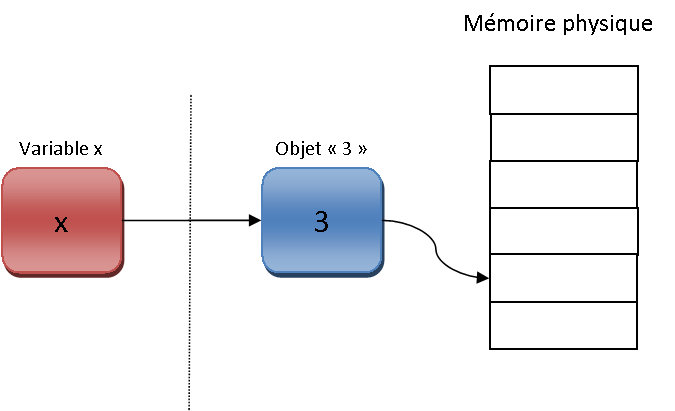
\includegraphics[width=0.45\textwidth]{img/affectation.png}
	\caption{Processus d'affectation d'une valeur à une variable. La variable x devient une référence de l'objet '3').}
	\label{fig:affectation}
\end{figure}

Cette association d'une variable à un objet est appelé \textbf{référence}. De manière imagée, on peut voir une variable comme une étiquette sur un objet. 

\underline{Remarque} : la fonction \lstinline{id()} permet de récupérer l'adresse mémoire d'un objet. Jouons avec cette fonction :
\begin{lstlisting}
>>> x = 3
>>> id(x)
19774651	# c'est l'adresse mémoire de a dans la table système
>>> y = "ensg"
>>> id(y)
23154984
>>> id(2)
56489413 # l'objet 2 possède une adresse mémoire même s'il n'est pas référencé par une variable
\end{lstlisting}

Sur chaque ordinateur les chiffres devraient être différents. Ce qui importe c'est de constater qu'ils sont tous différents. De même, on devrait observer que l'adresse mémoire d'un même objet est toujours identique :
\begin{lstlisting}
>>> x = 10
>>> id(y)
1446297760
>>> b = x
>>> id(y)
1446297760
>>> id(10)
1446297760
\end{lstlisting}

Python garde un objet en mémoire tant qu’il existe une référence vers cet objet :
\begin{lstlisting}
>>> x = 3
>>> y = x
>>> x = "a"	# x référence un nouvel objet "a"
>>> y
3						# la variable y référence toujours l'objet 3
>>> y = 5
\end{lstlisting}

Suite à la dernière ligne de l'exemple ci-dessus, l'objet 3 n'est plus référencé par aucune variable. Python va lancer un processus de nettoyage (aussi appelé \textit{garbage collector}) pour effacer cet objet de la mémoire. Voir illustration figure \ref{fig:garbage_collector}.

\begin{figure}
	\center 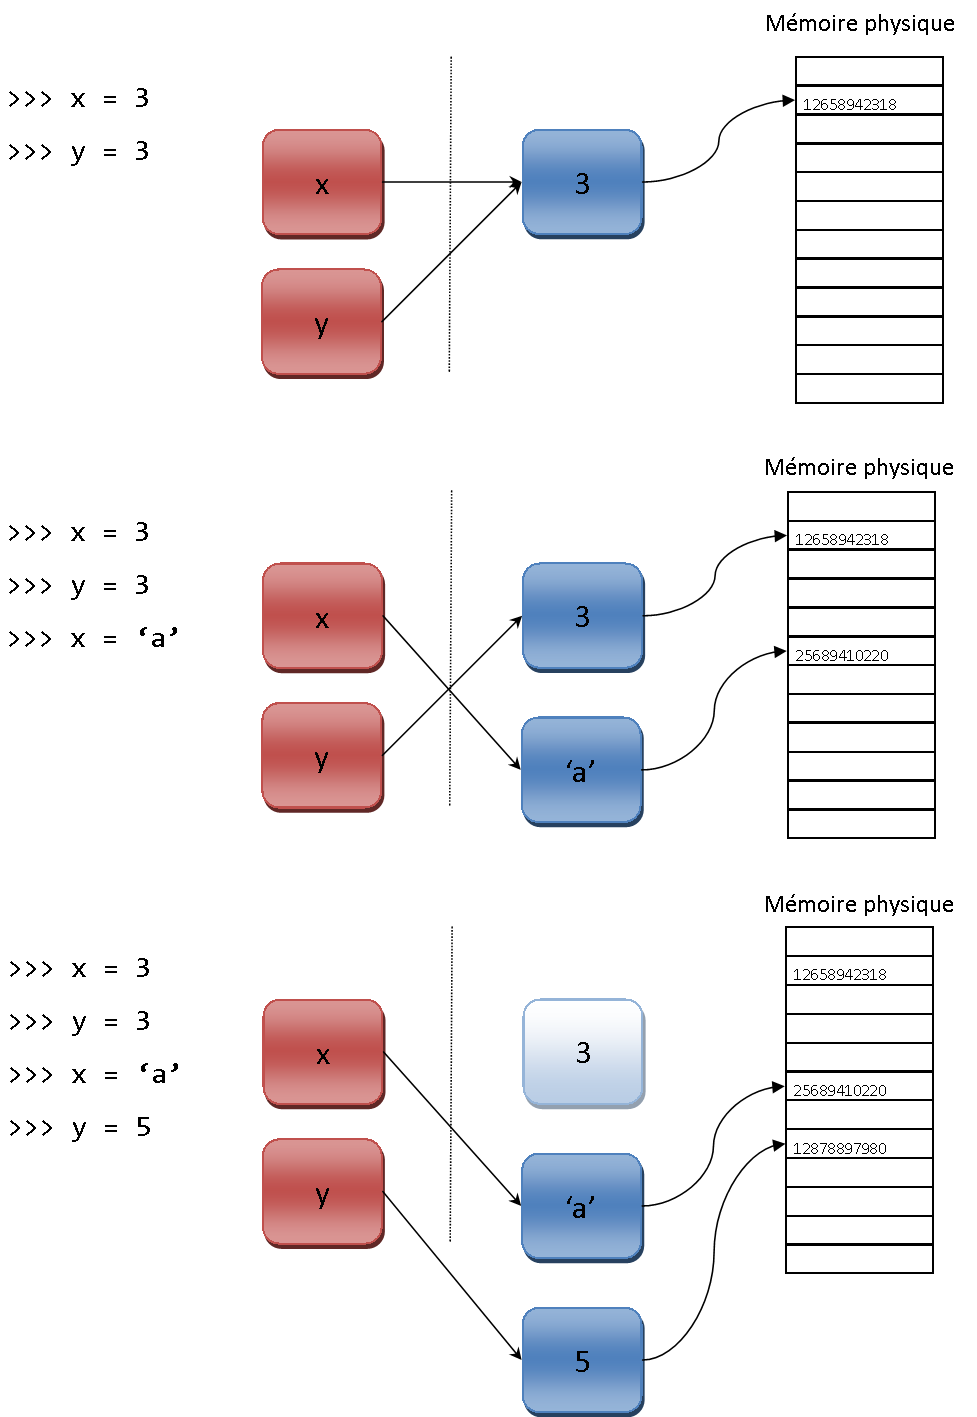
\includegraphics[width=0.55\textwidth]{img/garbage_collector.png}
	\caption{Illustration du processus de nettoyage lorsqu'une suite d'instructions est saisie.}
	\label{fig:garbage_collector}
\end{figure}

Un fois qu'un objet a été supprimé, si on en recrée un ayant la même valeur, il s’agira d'un nouvel objet différent du premier (son adresse mémoire est différente) :
\begin{lstlisting}
>>> x = "ensg"
>>> id(x)
47017920
>>> del(x)
>>> y = "ensg"
>>> id(y)
49017216
\end{lstlisting}

Pour conclure ce paragraphe, nous retiendrons :
\begin{itemize}
	\item qu'une variable est créée lorsqu'on lui affecte pour la première fois une valeur;
	\item qu'une variable n'est jamais associée à un type en Python. C'est l'objet qu'elle référence qui porte le type;
	\item qu'une variable est automatiquement remplacée par l'objet qu'elle référence dans une expression.
\end{itemize}


%%%
\subsection{Types de base}
Python met à disposition du programmeur un certain nombre de types ou structures de données. On parle de \textbf{types intégrés} (\textit{builtins}). Nous verrons au chapitre \ref{sec:poo} qu'il est également possible de définir ses propres structures de données.

Quel est donc l'intérêt d'utiliser les structures de données intégrés au langage ? 
Tout d'abord, nous remarquerons que ces types de base sont des composants naturels des structures manipulées dans les programmes (on manipule naturellement des entiers, des chaînes de caractères). Cela facilite donc grandement la programmation : il n'y a pas besoin de tout redéfinir pour chaque nouveau programme. Enfin, ces structures de données sont plus efficaces que des structures de données que l'on aurait reconstruites (les algorithmes ont été optimisés, écrit dans des langages performants comme le C).

\begin{table}[H]
	\begin{center}
		\begin{tabular}{l|l}
			\textbf{Type} & \textbf{Exemples de valeur} \\
			\hline
			Nombre & \lstinline{3, 1.1456, -3.5} \\
			Chaîne de caractère & \lstinline{'mot', 'petit texte'} \\
			Liste & \lstinline{[1, 2, 3], ['a', 'b'], ['a', 5, 2.3, 'f']} \\
			Tuple & \lstinline{(1, 3), ('a', 'b', 'c')} \\
			Ensemble & set('abc'), {'a', 'b', 'c'} \\
			Dictionnaire & {1:'a', 2:'b'} \\
			Fichier & \lstinline{open('fichier.txt')} \\
			Booléen & True, False \\
			Rien & \lstinline{None} \\
		\end{tabular}
		\caption{Types de base en Python}
		\label{tab:structure_donnees_base}
	\end{center}
\end{table}



%%% --------------------------
\section{Les types numériques}
\label{sec:types_numeriques}
Les nombres sont des objets relativement basiques et dont l'utilisation est assez naturelle.  Python inclus les types numériques "classiques", que l'on retrouve dans la plupart des langages de programmation : nombres entier, nombres à virgule; mais également d'autres moins courants : nombres complexes, nombres rationnels. Ces types couvrent la plupart des besoins standards.

\begin{table}[H]
	\begin{center}
		\begin{tabular}{|l|l|}
			\hline
			\textbf{Type} & \textbf{Exemple de valeur} \\
			\hline
			Integer & 2, -3, 156235789 \\
			Float &  2.3, -4.12, 1.0, 189489.23891\\
			Complex & 2 + 3j \\
			Decimal & Decimal('0.1') \\
			Fraction & Fraction(1, 3) \\
			\hline
		\end{tabular}
		\caption{Types numériques}
	\end{center}
\end{table}

\underline{Remarque} : les ensembles (cf. paragraphe \ref{sec:ensembles}) sont parfois comptés dans les types numériques car ils supportent les opérations mathématiques classiques : addition, soustraction, union, intersection...

Les nombres Python supportent les opérations mathématiques classiques listées dans la table \ref{tab:operateurs_numerique}. Dans le cas d'expression avec des parenthèses, Python applique la règle mathématique classique et calcule en premier les sous-expressions entre parenthèses.

\begin{table}[H]
	\begin{center}
		\begin{tabular}{|c|l|}
			\hline
			\textbf{Opérateur} & \textbf{Signification} \\
			\hline
			\lstinline{+} & Addition \\
			\lstinline{-} & Soustraction\\
			\lstinline{*} & Multiplication \\
			\lstinline{**} & Puissance \\
			\lstinline{/} & Division \\
			\lstinline{//} & Division entière \\
			\lstinline{%} & Reste d'une division entière (modulo) \\
			\hline
		\end{tabular}
		\caption{Opérateurs des types numériques}
		\label{tab:operateurs_numerique}
	\end{center}
\end{table}


%%%
\subsection{Nombres entiers et réels}
Python supporte les \textbf{nombres entiers} (\lstinline{int}) et les \textbf{nombres réels} (\lstinline{float}).
\begin{lstlisting}
>>> a = 3
>>> b = 3.0
>>> type(a)
<class 'int'>
>>> type(b)
<class 'float'>
\end{lstlisting}

Les fonctions \lstinline{int()} et \lstinline{float()} permettent de convertir un nombre quelconque en entier ou réel respectivement.
\begin{lstlisting}
>>> a = 3
>>> print(a)
3
>>> print(float(a))
3.0
>>> b = 3.0
>>> print(b)
3.0
>>> print(int(b))
3
\end{lstlisting}

Si les types sont mélangés au sein d'une même expression, Python convertit automatiquement le résultat vers le type le plus "complèxe".
\begin{lstlisting}
>>> 2 + 3.18
5.18
\end{lstlisting}

D'une manière générale, les opérations mathématiques complexes retournent systématiquement un réel\footnote{Nous reviendrons plus tard dans ce cours sur l'instruction import employée dans l'exemple. Nous l'utiliserons pour l'instant sans savoir ce qu'elle fait réellement.} :
\begin{lstlisting}
>>> import math
>>> math.cos(math.pi)
-1.0
\end{lstlisting}


%%%
\subsection{Nombres complexes}
Les \textbf{nombres complexes} sont gérés en standard en Python. Ils sont représentés en ajoutant un \lstinline{j} ou \lstinline{J} à la partie imaginaire du nombre complexe.
\begin{lstlisting}
>>> 1j * 1j
(-1+0j)
>>> 2 + 3j
(2+3j)
>>> 2j * (2 + 3j)
(-6+4j)
\end{lstlisting}

Attention, la syntaxe rend indispensable la présence du nombre devant le \lstinline{j} de la partie imaginaire, même s'il vaut 1. L'instruction \lstinline{j * j} retourne par exemple une erreur. C'est \lstinline{1j * 1j} qui est compris par Python.


%%%
\subsection{Autres types numériques}
Python possède également un type \textbf{Decimal} qui permet de gérer des nombres décimaux avec une précision définie par l'utilisateur. Cela est particulièrement utile dans les cas où la la conversion des nombres en binaires par la machine introduit des erreurs :
\begin{lstlisting}
>>> 0.1 + 0.1 + 0.1 - 0.3
5.551115123125783e-17
\end{lstlisting}

La syntaxe de création d'un nombre décimal est différentes des types précédents, puisqu'au lieu d'écrire un simple expression littérale, il faudra appeler une fonction.
\begin{lstlisting}
>>> from decimal import Decimal
>>> Decimal('0.1') + Decimal('0.1') + Decimal('0.1')  - Decimal('0.3')
Decimal('0.0')
>>> print(Decimal('0.1') + Decimal('0.1') + Decimal('0.1') - Decimal('0.3'))
0.0
\end{lstlisting}

Le type permet également de visualiser la valeur réellement stockée par l'ordinateur d'un nombre. Pour cela on n'utilise pas les apostrophes encadrant le nombre dans la fonction \lstinline{Decimal} :
\begin{lstlisting}
>>> Decimal('0.1')
Decimal('0.1')
>>> Decimal(0.1)
Decimal('0.1000000000000000055511151231257827021181583404541015625')
\end{lstlisting}

Enfin, les \textbf{nombres rationnels} (Fraction) ont été introduit en Python 2.6. Ils permettent de gérer des fractions sans perte de précision. La syntaxe est similaire à celle des nombres décimaux.
\begin{lstlisting}
>>> 1/6 + 1/2
0.6666666666666666
>>> from fractions import Fraction
>>> Fraction(1, 6) + Fraction(1, 2)
Fraction(2, 3)
\end{lstlisting}

Notons qu'il est toujours possible de revenir à une forme plus classique :
\begin{lstlisting}
>>> print(Fraction(1, 6) + Fraction(1, 2))
2/3
>>> float(Fraction(1, 6) + Fraction(1, 2))
0.6666666666666666
\end{lstlisting}

Des modules standards\footnote{Nous définirons précisément ce qu'est un module au chapitre \ref{sec:modules}}, comme \textit{math} étendent par ailleurs largement les opérations possible sur les types numériques (racine carrée, exponentielle, sinus, valeur absolue, etc.).


%%%
\subsection{Les booléens}
Pendant longtemps, Python n'a pas eu de type booléen et utilisait l'entier 0 pour faux et l'entier 1 pour vrai. Puis une sorte de sur-couche a été ajoutée à ces entiers 0 et 1 pour rendre le langage plus propre et permettre d'utiliser un vrai type booléen. Les valeurs \textbf{True} (vrai) et \textbf{False} (faux) sont les deux seules valeurs permises.
\begin{lstlisting}
>>> type(True)
<class 'bool'>
\end{lstlisting}

Concrètement, les booléens \lstinline{True} et \lstinline{False} ont le même comportement que les entiers 1 et 0, à l'exception que quelques méthodes qui ont été redéfinies (\lstinline{str} pour l'affichage par exemple). La plupart de opérations sur les types numériques sont donc compatibles avec les booléens.
\begin{lstlisting}
>>> True + 2
3
>>> float(False)
0.0
\end{lstlisting}

Si le booléen \lstinline{True} vaut 1, l'objet \lstinline{True} est bien un objet différent de 1 :
\begin{lstlisting}
>>> True == 1
True
>>> True is 1		# l'opérateur is compare les adresse mémoire des objets
False
\end{lstlisting}

Les opérations logiques retournent des booléens. La table \ref{tab:operateurs_comparaison} liste les opérateurs de comparaison. Ces opérateurs s'appliquent à tous les types de données, à condition que les types soient comparables (comparer 5 à "toto" n'a pas vraiment de sens).

\begin{table}[H]
	\begin{center}
		\begin{tabular}{|c|l|}
			\hline
			\textbf{Opérateur} & \textbf{Signification} \\
			\hline
			\lstinline{>} & Supérieur \\
			\lstinline{<} & Inférieur\\
			\lstinline{>=} & Supérieur ou égal \\
			\lstinline{<=} & Inférieur ou égal \\
			\lstinline{==} & Egal \\
			\lstinline{!=} ou \lstinline{<>} & Différent de \\
			\lstinline{is} & Objet identique \\
			\lstinline{is not} & Objet différent \\
			\hline
		\end{tabular}
	\caption{Opérateurs logiques}
	\label{tab:operateurs_comparaison}
	\end{center}
\end{table}

Dans l'exemple ci-dessous, nous affectons à x le résultat de la comparaison \lstinline{3 != 5}. Ce résultat est un booléen :
\begin{lstlisting}
>>> x = (3 != 5)
>>> x
True
\end{lstlisting}

Les expressions booléennes peuvent enfin être combinées entre elles à l'aide des mots clé \lstinline{and}, \lstinline{or} et \lstinline{not}. 

\begin{table}[H]
	\begin{center}
		\begin{tabular}{|c|l|}
			\hline
			\textbf{Opérateur} & \textbf{Signification} \\
			\hline
			\lstinline{X and Y} & Est vrai si X et Y sont vrai \\
			\lstinline{X or Y} & Est vrai si X ou Y est vrai\\
			\lstinline{not X} & Est vrai si X est faux \\
			\hline
		\end{tabular}
	\caption{Opérateurs booléens}
	\label{tab:operateurs_booleens}
	\end{center}
\end{table}

Exemple :
\begin{lstlisting}
>>> x = ((2 != 3) or (4 < 1)) and (not 5 == 2)
>>> x
True
\end{lstlisting}



%%% --------------------
\section{Le type "rien"}
Python propose un type spécial qui ne peut prendre qu'une seule valeur possible, \textbf{None}, et qui est utilisé pour signifier qu'une variable ne contient rien. Ou plus exactement, elle référence un objet et cet objet est l'objet "rien". 

Il s'agit d'une valeur qui est utilisée par défaut lorsqu'une opération n'a pas de retour explicite ou n'a pas pu être menée à son terme. Le type "rien" est ainsi utilisé pour vérifier que des parties de programme ont correctement fonctionné.

\begin{lstlisting}
>>> x = None
>>> x
>>> type(x)
<class 'NoneType'>
\end{lstlisting}



%%% -------------------------------
\section{Les chaînes de caractères}
Après avoir introduit les principaux types numériques, nous allons nous attarder sur un autre type de données fondamental : les \textbf{chaînes de caractères}. Une chaîne de caractères est définie comme une suite finie de caractères.

En Python, il n'existe qu'un seul type de données textuelles, qu'il s'agisse de caractère individuel, de mot ou de phrase ou de textes complets. Ce type est accompagné d'un nombre conséquent d'outils et de méthodes.

\subsection{Création d'une chaîne de caractères}
Les apostrophes et guillemets s'utilisent indifféremment pour définir une chaîne de caractères \lstinline{"..."} ou \lstinline{'...'} :
\begin{lstlisting}
>>> "demain" == 'demain'
True
\end{lstlisting}

L'intérêt d'utiliser l'une ou l'autre des deux formes est de pouvoir intégrer des apostrophes ou guillemets dans une chaîne :
\begin{lstlisting}
>>> "aujourd'hui", 'le type "rien"'
\end{lstlisting}

Si vous êtes amené à devoir utiliser des apostrophes au sein d'une chaîne définie à l'aide d'apostrophes, il vous faudra utiliser un anti-slash avant l'apostrophe à conserver dans la chaîne :
\begin{lstlisting}
>>> 'aujourd\'hui'
\end{lstlisting}

D'une manière plus générale, les anti-slashs sont utilisés pour signaler un caractère spécial :
\begin{itemize}
	\item \lstinline{\n} pour une nouvelle ligne;
	\item \lstinline{\t} pour une tabulation;
	\item \lstinline{\\} pour un anti-slashe;
	\item etc.
\end{itemize}

Nous remarquerons que cette syntaxe n'est pas des plus pratiques lorsqu'il s'agit d'enregistrer un chemin d'accès. Par exemple, \lstinline{'C:\nouvel_an\photos\tri'} ne va pas être lu correctement par Python (un retour à la ligne et une tabulation remplaceront les \lstinline{\n} \lstinline{\t}). Aussi, pour simplifier l'écriture des chaînes de caractères comportant beaucoup de caractères spéciaux, Python propose d'utiliser une syntaxe qui va interpréter les \lstinline{\} comme de simples \lstinline{\} : les \textit{raw strings}.

Si un \lstinline{'r'} apparaît juste devant une chaîne de caractère, les caractères sont interprétés comme ils apparaissent :
\begin{lstlisting}
>>> print('C:\nouvel_an\photos\tri')
C:
ouvel_an\photos    ri
>>> print(r'C:\nouvel_an\photos\tri')
C:\nouvel_an\photos\tri
\end{lstlisting}

Python propose un troisième mode de définition de chaînes de caractères qui commence et se termine par trois guillemets : \lstinline{"""..."""}. Cette syntaxe permet de conserver la mise en forme d'un bloc de texte.
\begin{lstlisting}
>>> """Les trois quotes :
permettant d'enregistrer la mise en forme.

     => y compris les sauts de ligne, les tabulations..."""
"Les trois quotes :\npermettant d'enregistrer la mise en forme.\n\n\t=> y compris les sauts de ligne, les tabulations..."
\end{lstlisting}


%%%
\subsection{Manipulation d'un chaîne de caractères}
Les chaînes de caractères supportent de nombreuses opérations : tester la présence d'un caractère ou d'un groupe de caractères dans une chaîne, accéder à un caractère à partir de sa position dans la chaîne, compter la longueur de la chaîne, etc. La table \ref{tab:operateurs_chaines} liste les principaux opérateurs applicables aux chaînes de caractères tandis que la table \ref{tab:fonctions_chaines} recense quelques fonctions s'appliquant sur ces chaînes. La syntaxe générale des fonctions s'appliquant aux chaînes de caractères est : \lstinline{resultat = chaine.fonction(...)}.

\begin{table}[H]
	\begin{center}
		\begin{tabular}{|c|l|}
			\hline
			\textbf{Opérateur} & \textbf{Signification} \\
			\hline
			\lstinline{+} & Concaténation de chaînes de caractères \\
			\lstinline{*} & Répétition d'une chaîne de caractères \\
			\lstinline{in} & Inclusion d'une chaîne dans une autre \\
			\lstinline{not in} & Non inclusion d'une chaîne dans une autre \\
			\lstinline{[i]} & Caractère à la i-ième position dans la chaîne \\
			\lstinline{[i:j]} & Caractères compris entre les i-ième et j-ième positions \\
			\hline
		\end{tabular}
		\caption{Opérateurs du type chaîne de caractères}
		\label{tab:operateurs_chaines}
	\end{center}
\end{table}

\begin{table}[H]
	\begin{center}
		\begin{tabular}{|l|p{11cm}|}
			\hline
			\textbf{Fonction} & \textbf{Signification} \\
			\hline
			\lstinline{chaine.count(s)} & Compte le nombre d’occurrence du caractère \lstinline{s} (ou chaîne de caractères \lstinline{s})\\
			\lstinline{chaine.find(s)} & Retourne l'indice de la première occurrence de \lstinline{s} dans la chaîne ou -1 si elle n'est pas présente \\
			\lstinline{chaine.isalpha()} & Retourne \lstinline{True} si la chaîne est composée exclusivement de lettres \\
			\lstinline{chaine.isdigit()} & Retourne \lstinline{True} si la chaîne est composée exclusivement de chiffres \\
			\lstinline{chaine.replace(old, new)} & Retourne un copie de la chaîne où les caractères \lstinline{old} ont été remplacés par \lstinline{new} \\
			\lstinline{chaine.split(sep)} & Découpe la chaîne en se servant de \lstinline{sep} comme délimiteur \\
			\lstinline{chaine.strip(s)} & Supprime les espaces au début et à la fin de chaîne. Supprime aussi \lstinline{s} s'il est renseigné \\
			\lstinline{chaine.upper()} & Remplace les minuscules par des majuscules \\
			\lstinline{chaine.string.lower()} & Remplace les majuscules par des minuscules \\
			\lstinline{chaine.capitalize()} & Met en majuscule la première lettre \\
			\lstinline{chaine.endwith(s)} & Retourne vrai si la chaîne se termine par les caractères \lstinline{s} \\
			\lstinline{chaine.startwith(s)} & Retourne vrai si la chaîne commence par les caractères \lstinline{s} \\
			\hline
		\end{tabular}
		\caption{Fonctions s'appliquant aux chaînes de caractère}
		\label{tab:fonctions_chaines}
	\end{center}
\end{table}

Il est possible de convertir le contenu d'une variable quelconque en chaîne de caractère en utilisant la fonction \lstinline{str()}. 
\begin{lstlisting}
>>> a = 2.1745
>>> b = str(a)
>>> type(b)
<class 'str'>
\end{lstlisting}

La fonction \lstinline{len()} retourne la longueur de la chaîne de caractère.
\begin{lstlisting}
>>> a = "ensg"
>>> len(a)
4
\end{lstlisting}

Dans l'exemple suivant, nous montrons que la concaténation de deux chaînes de caractères entraîne la création d'un nouvel objet de type chaîne de caractère. Puis nous utilisons la fonction \lstinline{replace()} pour remplacer des caractères. Là encore un nouvel objet est créé. Plus généralement, les chaînes de caractères ne peuvent pas être modifiées, on dit qu'elles sont immuables.
\begin{lstlisting}
>>> txt = "Boum"
>>> id(txt)
44826144
>>> txt = txt + "!"
>>> txt
"Boum!"
>>> id(txt)
44768576          # il ne s'agit plus du même objet. La concaténation crée un nouvel objet.
>>> txt = txt.replace("ou", "a")
>>> txt
"Bam!"
>>> id(txt)
44766304          # il s'agit bien d'un nouvel objet
\end{lstlisting}


%%%
\subsection{Formatage de texte}
Python offre plusieurs possibilités de formatage de chaînes de caractères qui sont utiles pour afficher les valeurs contenues dans les variables. Deux syntaxes existent depuis la version 2.6 de Python. La syntaxe originale :
\begin{lstlisting}
>>> "... %c ..." % (valeur)
\end{lstlisting}

Le format est indiqué après le premier symbole \% sous la forme d'une lettre correspondant un type de formatage. La valeur est elle indiquée en fin de ligne après le second symbole \%. Il est possible de formater plusieurs chaînes en même temps : 
\begin{lstlisting}
>>> "...%c1...%c2..." % (v1, v2)
\end{lstlisting}

Les valeurs courantes des codes de formatage sont les suivantes :
\begin{itemize}
	\item s texte simple (résultat de la fonction str(v))
	\item i nombre entier
	\item e nombre réel au format exponentiel
	\item f nombre réel au format décimal
\end{itemize}

La précision du formatage peut être précisée entre le \% et le code. La syntaxe générale est \lstinline{%[align][largeur][.precision][code]} :
\begin{lstlisting}
>>> n = 3.2547
>>> 'n = %s' %(n)
'n = 3.2547'
>>> 'n = %15s' %(n)
'n =          3.2547'
>>> 'n = %f' %(n)
'n = 3.254700'
>>> 'n = %.2f' %(n)
'n = 3.25'
\end{lstlisting}

L'autre syntaxe est la suivante :
\begin{lstlisting}
>>> "...{}...".format(valeur)
\end{lstlisting}

Il est également possible de formater plusieurs chaînes simultanément :
\begin{lstlisting}
>>> "...{}...{}...".format(v1, v2)
\end{lstlisting}

Et le format de sortie peut aussi être spécifié :
\begin{lstlisting}
>>> "...{:c}...".format(valeur)
\end{lstlisting}

Les codes de formatage sont identiques à ceux de la première forme présentée.

\underline{Remarque} : pour la très grande majorité des usages, les deux méthodes sont équivalentes. Excepté pour des usages avancés dépassant le cadre de ce cours, le choix de l'une ou l'autre n'aura pas d'importance.



%%% -------------------
\section{Les séquences}
\label{sec:sequences}
Les séquences ne sont pas un type de données à proprement parler mais plutôt une catégorie qui regroupe un ensembles de structures de données partageant des propriétés communes. Python dispose de trois types "basiques" de séquences : \lstinline{list}, \lstinline{tuple} et \lstinline{range}. Les chaînes de caractères (\lstinline{string}, introduites partie précédente) constituent également un type particulier de séquences.

Nous commencerons par évoquer les aspects communs à toutes les séquences puis nous détaillerons les spécificités de chacune.


%%%
\subsection{Généralités sur les séquences}
Les séquences partagent en commun le fait d'être \textbf{itérables} et \textbf{indexables}. Cela signifie que :
\begin{itemize}
	\item une séquence est capable de retourner les éléments qui la composent les uns à la suite des autres (=itérable);
	\item une séquence est capable de retourner n'importe lequel de ses éléments sans avoir à parcourir l'ensemble de la séquence (=indexable).
\end{itemize}

Les chaînes de caractères étudiées au chapitre précédent sont un exemple de séquence. Il est en effet possible de récupérer une lettre par son indice dans la chaîne :
\begin{lstlisting}
>>> s = 'abracabra'
>>> s[3]		# 3ème élément de s
'a'
\end{lstlisting}

Nous en profitons pour remarquer que l'indexation d'une séquence commence à 0 : \lstinline{s[0] = 'a'}

Il est également possible de parcourir la chaîne caractère par caractère\footnote{L'exemple utilise des fonctions \lstinline{iter()} et \lstinline{next()} qui ne sont pas à connaître et sur lesquelles nous reviendrons ultérieurement} :
\begin{lstlisting}
>>> s = 'abracabra'
>>> iterateur = iter(s)	# on se prépare à parcourir s
>>> next(iterateur)	# on se positionne sur le premier élément de s
'a'
>>> next(iterateur)	# on passe au suivant
'b'
>>> next(iterateur)	# on passe au suivant...
'r'
\end{lstlisting}

Nous distinguerons deux grandes catégories de séquences :
\begin{itemize}
	\item les \textbf{séquences immuables} ne supportent pas la modification de leurs éléments;
	\item les \textbf{séquences modifiables} (ou mutables) peuvent voir leurs éléments modifiés sans avoir à être redéfinies.
\end{itemize}

Toutes les séquences supportent les opérations répertoriées dans la table \ref{tab:operateurs_sequences}. Les chaînes de caractères étant des séquences, les opérations listées dans cette table recoupent celles déjà listées dans la table \ref{tab:operateurs_chaines}.
\begin{table}[H]
	\begin{center}
		\begin{tabular}{|l|p{11cm}|}
			\hline
			\textbf{Opérateur} & \textbf{Signification} \\
			\hline
			\lstinline{x in s} & x est dans s \\
			\lstinline{x not in s} & x n'est pas dans s \\
			\lstinline{s + t} & concaténation de s et t \\
			\lstinline{s * n} & ajouter n fois s à lui-même \\
			\lstinline{s[i]} & élément à la i-ème position \\
			\lstinline{s[i:j]}  & sous-séquence de s, de la i-ème à la j-ème position \\
			\lstinline{s[i:j:k]} & sous-séquence de s, de la i-ème à la j-ème position avec un pas de k \\
			\lstinline{len(s)}  & nombre d'éléments de la séquence s \\
			\lstinline{min(s)}  & plus petit élément de la séquence s (lorsque cela à un sens) \\
			\lstinline{max(s)}  & plus grand élément de la séquence s (lorsque cela à un sens) \\
			\lstinline{sum(s)}  & somme des éléments de la séquence s (lorsque cela à un sens) \\
			\lstinline{s.index(x, i, j)}  & index de la première occurence de x dans s, à partir de l'indice i et jusqu'à j \\
			\lstinline{s.count(x)}  & nombre d'occurence de x dans s \\
			\hline
		\end{tabular}
		\caption{Opérateurs sur les séquences}
		\label{tab:operateurs_sequences}
	\end{center}
\end{table}



%%%
\subsection{Les tuples}
Un \textbf{tuple} est un tableau d'objets qui peuvent être de n'importe quel type. Les tuples, comme les chaînes de caractères ou les numériques, ne sont pas modifiables : ce sont des \textit{séquences immuables}.

Pour créer un tuple, on sépare les différentes valeurs qui vont le composer par des virgules :
\begin{lstlisting}
>>> t = 2016, "ENSG", 'Géomatique'
>>> type(t)
<class 'tuple'>
>>> t
(2016, 'ENSG', 'Géomatique')
\end{lstlisting}

Pour améliorer la lecture du code, on utilise souvent des parenthèses lors de la définition d'un tuple :
\begin{lstlisting}
>>> t = (2016, "ENSG", 'Géomatique')
\end{lstlisting}

Les tuples peuvent être imbriqués :
\begin{lstlisting}
>>> t, (1, 2, 3, 4)
((2016, 'ENSG', 'Géomatique'), (1, 2, 3, 4))
\end{lstlisting}

Les tuples sont toujours représentés entre parenthèses. Comme pour une chaîne de caractère, il est impossible de modifier la valeur d'un élément d'un tuple.
\begin{lstlisting}
>>> t = 2016, 'ENSG', 'Géomatique'
>>> t[0] = 2017
TypeError: 'tuple' object does not support item assignement
\end{lstlisting}

Tous les opérateurs définis dans le paragraphe de généralités sur les séquences s'appliquent bien entendu aux tuples.

\underline{Remarque} : pour créer un tuple de zéro ou un élément, on utilise une subtilité de la syntaxe :
\begin{lstlisting}
>>> t = ()     # crée un tuple vide
>>> t
()
>>> t = 1,     # crée un tuple de un élément
>>> t
(1,)
\end{lstlisting}
Mais attention, utiliser les parenthèses sans virgule ne fonctionne pas :
\begin{lstlisting}
>>> t = (15)     # crée un entier
>>> type(t)
<class 'int'>
\end{lstlisting}


%%%
\subsection{Les listes}
Une \textbf{liste} est similaire à un tuple à la différence près qu'il est possible de modifier, ajouter ou supprimer des éléments d'une liste sans avoir à la redéfinir : les listes sont des \textit{séquences modifiables}. 

Tous les opérateurs définit pour les séquences seront utilisable sur les listes (cf. table \ref{tab:operateurs_sequences}). Mais du fait de leur caractère modifiable, elles supporteront des opérateurs supplémentaires listés dans le table \ref{tab:operateurs_listes} (opérateurs par ailleurs communs à tous les types de séquences modifiables).

Une liste est définit par un ensemble de valeurs entre deux crochets :
\begin{lstlisting}
>>> a = [2016, "ENSG", 'Géomatique']
>>> type(a)
<class 'list'>
>>> a
[2016, 'ENSG', 'Géomatique']
\end{lstlisting}

Les listes peuvent également être imbriquées :
\begin{lstlisting}
>>> b = [a, [1, 2, 3, 4]]
>>> b
[[2016, 'ENSG', 'Géomatique'], [1, 2, 3, 4]]
\end{lstlisting}

Pour créer une liste vide, nous utilisons des crochets sans rien à l'intérieur :
\begin{lstlisting}
>>> c = []
>>> type(c)
<class 'list'>
\end{lstlisting}

\begin{table}[H]
	\begin{center}
		\begin{tabular}{|l|p{11cm}|}
			\hline
			\textbf{Opérateur} & \textbf{Signification} \\
			\hline
			\lstinline{L[i] = x} & Elément à la position i remplacé par x \\
			\lstinline{L[i:j] = t} & Partie entre les position i et j remplacé par la liste t \\
			\lstinline{del(L[i:j])} & Suppression des éléments entre les positions i et j. Equivalent à \lstinline{L[i:j] = []} \\
			\lstinline{L[i:j:k] = t} & Partie entre les position i et j avec un pas de k remplacé par la liste t \\
			\lstinline{del(L[i:j:k])} & Suppression des éléments entre les positions i et j avec un pas de k. Equivalent à \lstinline{L[i:j:k] = []} \\
			\lstinline{L += t} & Ajoute t à L \\
			\lstinline{L *= n}  & Ajoute n-1 fois L à elle-même \\
			\hline
		\end{tabular}
		\caption{Opérateurs sur les listes}
		\label{tab:operateurs_listes}
	\end{center}
\end{table}

Du fait de leur caractère modifiables, un certains nombres de fonctions viennent avec les listes (cf. table \ref{tab:fonctions_listes}).

\begin{table}[H]
	\begin{center}
		\begin{tabular}{|l|p{11cm}|}
			\hline
			\textbf{Fonction} & \textbf{Signification} \\
			\hline
			\lstinline{l.append(x)} & Ajoute l'élément \lstinline{x} à la fin de la liste \\
			\lstinline{l.extend(t)} ou \lstinline{l += t} & Ajoute les éléments de la liste \lstinline{t} en fin de liste \lstinline{l} \\
			\lstinline{l.insert(i, x)} & Insertion de l'élément x à la position i \\
			\lstinline{l.remove(x)} & Suppression de tous les éléments x \\
			\lstinline{l.pop(i)} & Retourne et supprime de la liste l'élément à la position i \\
			\lstinline{l.clear()} & Vide la liste \\
			\lstinline{l.reverse()} & Inverse l'ordre des éléments de la liste \\
			\lstinline{l.copy()} & Crée une copie de la liste \\
			\lstinline{l.sort()} & Trie les éléments de la liste par ordre croissant\footnote{La fonction sort() s'applique uniquement aux listes, et non à l'ensemble des séquences modifiables.} \\
			\hline
		\end{tabular}
		\caption{Fonctions s'appliquant listes}
		\label{tab:fonctions_listes}
	\end{center}
\end{table}

%\underline{Remarque} : il est possible d'utiliser une liste Python comme une pile ou une file.

\underline{Remarque} : les nombres entiers et flottants sont généralement compatibles et gérés automatiquement par Python (cf. partie \label{sec:types_numeriques}). L'une des rares exceptions à cette compatibilité est leur utilisation comme index de listes où seuls les entiers sont acceptés.
\begin{lstlisting}
>>> liste = [0, 1, 2, 3, 4, 5]
>>> liste[5]
5
>>> liste[5.0]
TypeError: list indices must be integers, not float
\end{lstlisting}


%%%
\subsection{Les ranges}
Les ranges sont des séquences immuables de nombres entiers. Elles sont définies à l'aide d'une borne finale et éventuellement d'une borne initiale et d'un pas. Si la borne initiale est omise, la valeur par défaut sera zéro. Le pas par défaut vaut quant à lui 1.
\begin{lstlisting}
>>> a = range(10)
>>> type(a)
<class 'range'>
\end{lstlisting}

Pour visualiser le contenu d'un objet de type \lstinline{range}, on le convertit en liste à l'aide de la fonction \lstinline{list()} :
\begin{lstlisting}
>>> a = list(range(10))
>>> a
[0, 1, 2, 3, 4, 5, 6, 7, 8, 9]
>>> b = list(range(2, 10))
>>> b
[2, 3, 4, 5, 6, 7, 8, 9]
>>> c = list(range(2, 10, 2))
>>> c
[2, 4, 6, 8]
\end{lstlisting}

Les \lstinline{range} sont couramment utilisés comme compteur dans les boucles \lstinline{for} (cf. chapitre \ref{sec:boucles}).



%%% -----------------------
\section{Les dictionnaires}
Les \textbf{dictionnaires} sont des objets semblables aux listes mais plus souple en ce qui concerne le référencement des valeurs. Alors qu'une liste référence les éléments qu'elle contient à l'aide de leur position (un entier compris entre 0 et la taille de la liste), un dictionnaire se contente d'associer l'élément à un autre élément de type immuable (entier, réel, chaîne, tuple). On dit que le dictionnaire \textit{associe une valeur à une clé}.

Les éléments d'un dictionnaire \textit{ne sont pas ordonnés} (il n'est pas possible de les trier) et on y accède uniquement par leurs clés. La structure d'un dictionnaire n'est pas figée, on peut ajouter/modifier/supprimer des éléments sans avoir besoin de recréer le dictionnaire : le dictionnaire est \textit{modifiable}.

La syntaxe de création d'un dictionnaire est la suivante :
\begin{lstlisting}
>>> dico = {cle1: valeur1, cle2: valeur2...}
\end{lstlisting}

On peut créer un dictionnaire vide : 
\begin{lstlisting}
>>> dico = {}
>>> dico = dict()
\end{lstlisting}

Pour accéder à la valeur d'un élément, la syntaxe est semblable à celle d'une liste, mais l'indice n'est plus uniquement un entier : \lstinline{dico[cle]} retourne la valeur associé à la clé.
\begin{lstlisting}
>>> dico = {'prenom': 'paul', 'age': 24}
>>> dico['prenom']
'paul'
\end{lstlisting}

L'ajout d'une nouvel élément est assez aisé :
\begin{lstlisting}
>>> dico[0] = 'rouge'
>>> dico
{0: 'rouge', 'age': 24, 'prenom': 'paul'}
\end{lstlisting}

Les autres opérations et méthodes pour les dictionnaires sont listées respectivement dans les tables \ref{tab:operateurs_dictionnaires} et \ref{tab:fonctions_dictionnaires}.

\begin{table}[H]
	\begin{center}
		\begin{tabular}{|c|l|}
			\hline
			\textbf{Opérateur} & \textbf{Signification} \\
			\hline
			\lstinline{x in d} & x est dans une des clés de d \\
			\lstinline{x not in d} & x n'est pas dans les clés de d \\
			\lstinline{d[c]} & retourne l'élément associé à la clé c \\
			\lstinline{len(d)}  & nombre d'éléments de d \\
			\lstinline{del(d[c]}  & supprime l'élément associé à la clé c \\
			\hline
		\end{tabular}
		\caption{Opérateurs sur les dictionnaires}
		\label{tab:operateurs_dictionnaires}
	\end{center}
\end{table}

\begin{table}[H]
	\begin{center}
		\begin{tabular}{|l|l|}
			\hline
			\textbf{Fonction} & \textbf{Signification} \\
			\hline
			\lstinline{d.has_key(x)} & retourne vrai si x est une clé \\
			\lstinline{d.items()} & retourne une liste des couples (clé, valeur) du dictionnaire \\
			\lstinline{d.keys()} & retourne une liste des clés du dictionnaire \\
			\lstinline{d.values()}  & retourne une liste des valeurs du dictionnaire \\
			\lstinline{d.update(dico2)}  & dico reçoit le contenu de dico2 \\
			\lstinline{d.clear()}  & vide le dictionnaire \\
			\hline
		\end{tabular}
		\caption{Fonctions disponibles pour les dictionnaires}
		\label{tab:fonctions_dictionnaires}
	\end{center}
\end{table}



%%%--------------------
\section{Les ensembles}
\label{sec:ensembles}
Les ensembles (\lstinline{set}) sont des collections non ordonnées d'objets. Ils possèdent des propriétés communes avec les listes ou les dictionnaires, et sont également proches sur certains points des types numériques. Les ensembles :
\begin{itemize}
	\item sont itérables : il est possible de retourner les éléments qui les composent les uns à la suite des autres);
	\item sont modifiables (supportent les ajouts/suppressions d'éléments);
	\item peuvent contenir tous types d'objets;
	\item supportent les propriétés mathématiques des ensembles (union, intersection, etc.; cf. table \ref{tab:operateurs_ensembles}).
\end{itemize}

Mais les ensembles :
\begin{itemize}
	\item sont pas indexables : il est impossible de récupérer un élément à partir d'une position;
	\item ne contiennent pas d'objets en double.
\end{itemize}

\begin{table}[H]
	\begin{center}
		\begin{tabular}{|c|l|}
			\hline
			\textbf{Opérateur} & \textbf{Signification} \\
			\hline
			\lstinline{|} & Union \\
			\lstinline{&} & Intersection\\
			\lstinline{-} & Différence \\
			\lstinline{^} & Différence symétrique \\
			\hline
		\end{tabular}
		\caption{Opérateurs des ensembles}
		\label{tab:operateurs_ensembles}
	\end{center}
\end{table}

On définit un ensemble soit à l'aide du mot clé \lstinline{set} soit entre acolades : 
\begin{lstlisting}
>>> a = set('abracadabra')
>>> type(a)
<class 'set'>
>>> a
{'c', 'r', 'd', 'a', 'b'}  # les doublons ont disparus
>>> b = {'a', 'l', 'a', 'c', 'a', 'z', 'a', 'm'}
>>> type(b)
<class 'set'>
>>> b
{'m', 'c', 'z', 'l', 'a'}
\end{lstlisting}

Comme les autres collections déjà introduites, les ensembles supportent les opérations \lstinline{x in set}ou \lstinline{len(set)} et les fonctions \lstinline{add(x)}, \lstinline{remove(x)} ou encore \lstinline{pop()}.
\begin{lstlisting}
>>> a & b 
{'c', 'a'}
>>> a ^ b
{'l', 'b', 'd', 'm', 'z', 'r'}
>>> a.add(14)
>>> a
{'b', 14, 'd', 'c', 'r', 'a'}
\end{lstlisting}

Si on essaye d'ajouter un élément déjà présent dans un ensemble, Python le détecte et ne fait rien :
\begin{lstlisting}
>>> a.add(14)
>>> a
{'b', 14, 'd', 'c', 'r', 'a'}
\end{lstlisting}



%%% ------------------
\section{Les fichiers}
\label{sec:fichiers}
Dans ce paragraphe, nous nous attarderons sur le dernier type de base qui sera présenté dans ce cours : les fichiers. Nous montrerons comment lire ou écrire dans un fichier.

% Ce chapitre fait appel à plusieurs reprise à des notions qui n'ont pas encore été introduites dans ce cours. Cela n'empèche normalement pas la lecture et la compréhension des opérations sur les fichiers dont il est question ici et qui sont capitales en programmation. Si le lecteur était perturbé par certain points, nous lui conseillons de revenir ici ultérieurement.

%%%
\subsection{Chemins d'accès aux fichiers}
Avant de commencer à manipuler  les fichiers, précisons qu'il existe deux possibilités pour parcourir l'arborescence d'un système : utiliser des chemins \textit{absolus} ou \textit{relatifs}. 

Lorsque l'on utilise des chemins absolus, on décrit le fichier en partant de la racine du disque. Les chemins prennent la forme : \lstinline{D:\Exercices Python\resultat.txt}. 

Avec les chemins relatifs, on tiens compte du répertoire courant, c'est à dire celui depuis lequel l'interpréteur Python est exécuté (si l'on exécute un fichier .py directement, le répertoire courant est celui contenant le programme; si on utilise l'interpréteur Python, le répertoire courant est celui contenant l'interpréteur). Ainsi, si on est dans le répertoire \lstinline{D:\Exercice Python}, on appellera la fichier \lstinline{resultat.txt} de ce répertoire en saisissant tout simplement \lstinline{resultat.txt}.

\underline{Remarque} : il arrive parfois que l'on ne sache pas quelle est le répertoire courant. Pour le connaître on peut utiliser la commande \lstinline{os.getcwd()}. Il arrivera également qu'il faille changer de répertoire courant. On utilisera alors la commande \lstinline{os.chdir(repertoire)}.


%%%
\subsection{Ouverture d'un fichier}
Pour ouvrir un fichier, on utilise la fonction \lstinline{open()}. Elle prend en paramètre :
\begin{itemize}
	\item le chemin du fichier;
	\item le mode d'ouverture :
	\begin{itemize}
		\item \lstinline{'r'} pour lire uniquement;
		\item \lstinline{'w'} pour écrire uniquement (le contenu précédent est écrasé);
		\item \lstinline{'a'} pour lire et écrire à la fin (le contenu précédent est conservé);
	\end{itemize}
\end{itemize}

Il est possible de combiner les modes pour, par exemple, lire et ajouter à la fin.

Lorsque le fichier n'est plus utilisé par le programme, il est nécessaire de le fermer, sans quoi un verrou persiste empêchant son utilisation par une autre personne. On utilise la fonction \lstinline{close()}.


%%%
\subsection{Lecture d'un fichier}
Plusieurs modes de lecture d'un fichier sont possible. Les plus courants sont :
\begin{itemize}
	\item la lecture en entier avec la fonction \lstinline{read()}
	\item la lecture ligne par ligne avec la fonction \lstinline{readlines()}
\end{itemize}

D'autres modes permettent la lecture bit par bit ou caractère par caractère.

Un exemple de lecture :
\begin{lstlisting}
>>> fichier = open("fichier.txt", 'r')
>>> contenu = fichier.read()
>>> fichier.close()
>>> print(contenu)
Je suis le contenu d'un fichier texte !
\end{lstlisting}


%%%
\subsection{Ecriture dans un fichier}
Pour écrire dans un fichier, on utilise la méthode \lstinline{write(texte)} en lui passant en paramètre la chaîne de caractères à écrire. Elle renvoie le nombre de caractères qui ont été écrits. Cette fonction peut être appelées plusieurs fois pour écrire plusieurs chaînes. Elle fonctionne que le fichier soit ouvert en mode \lstinline{'w'} ou \lstinline{'a'}.
\begin{lstlisting}
>>> fichier = open("fichier.txt", 'w')
>>> fichier.write("J'écris pour la première fois dans un fichier texte via Python")
62
>>> fichier.close()
\end{lstlisting}


%%%
\subsection{L'ouverture avec \lstinline{with}}
L'ouverture et la manipulation de fichiers est une opération source d'erreurs en programmation. De plus, il est facile d'oublier de refermer un fichier après son utilisation, ce qui peut être problématique également.

Pour simplifier l'utilisation des fichiers, Python permet d'utiliser un mot clé \lstinline{with}. Avec cette forme d'ouverture d'un fichier, la fermeture du fichier est automatique :
\begin{lstlisting}
>>> with open("fichier.txt", 'r') as fichier:
...     contenu = fichier.read()
...     print(contenu)
...
Je suis le contenu d'un fichier texte !
\end{lstlisting}




%%% ------------
%\section{Résumé}
%hiérarchie des types : nombres / séquences / dictionnaires
%
%types modifiables / immuables



%%% ------------------
%%% Syntaxe du langage
%%% ------------------
\newpage
\part{Syntaxe du langage}
\chapter{}
Au chapitre précédent, nous avons étudié les structures de base intégrées dans le langage Python. Maintenant que nous maîtrisons les différents types de données, nous pouvons commencer à construire nos premières expressions en Python. 

Dans ce chapitre, nous allons commencer par rappeler les règles générales de construction des expressions en Python, puis nous apprendrons à construire les structures élémentaires du langage.


%%% ---------------------------------
\section{Structure du code en Python}
En Python, la règle générale est que la fin d'un ligne correspond à la fin d'une instruction\footnote{Il est toutefois possible d'écrire une instruction sur plusieurs lignes s'il s'agit d'une expression entre parenthèse, crochet, accolade. On utilise cette possibilité pour limiter la taille des grandes instructions et faciliter la lecture}. Il n'y a pas de symbole de fin d'instruction comme dans d'autres langages.

L'exemple suivant en Java :
\begin{lstlisting}
instruction1 ;
instruction2 ;
\end{lstlisting}

S'écrit simplement comme suit en Python :
\begin{lstlisting}
instruction1
instruction2
\end{lstlisting}

Pour définir un bloc de code, Python utilise l'indentation. De plus la ligne d'en tête du bloc se termine par deux points (\lstinline{:}). Ce qui donne :
\begin{lstlisting}
ligne_d_en_tete:
		bloc_d_instructions
\end{lstlisting}

La fin de l'indentation correspond à la fin du bloc d'instructions. Il n'est pas nécessaire d'ajouter un symbole spécial pour marquer la fin du bloc. On n'utilise pas non plus d'accolades pour délimiter le bloc d'instructions.

Par exemple, un test qui en Java aurait la forme :
\begin{lstlisting}
if (condition) {
		instruction1
		instruction2
}
\end{lstlisting}

S'écrirait en Python :
\begin{lstlisting}
if condition:
		instruction1
		instruction2

\end{lstlisting}

Ces quelques règles assurent une certaine homogénéité du code entre différents programmeurs : il n'y pas pas de risque de voir des développeurs écrire plusieurs instructions sur la même ligne, indenter ou pas leurs codes, etc. La figure \ref{img:structure_code} représente de manière imagée la structure d'un programme Python.

\begin{figure}[H]
	\center 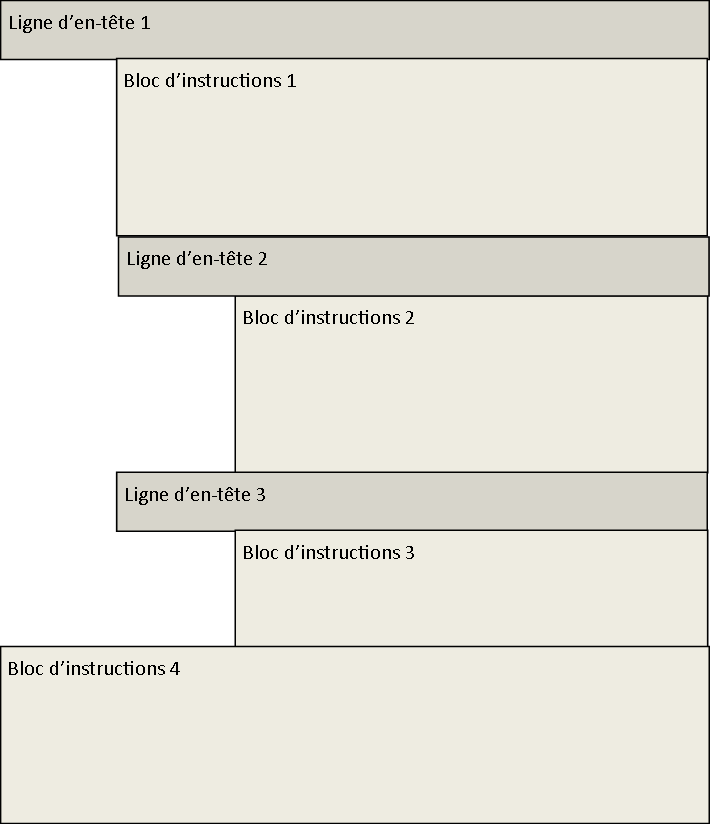
\includegraphics[width=200px]{img/structure_code_python.png}
	\caption{Structure du code en Python}
	\label{img:structure_code}
\end{figure}
	
	
Notons également que les espaces et sauts de ligne sont ignorés par l'interpréteur Python.
\begin{lstlisting}
ligne_d_en_tete:
		instruction1
instruction2
\end{lstlisting}

Est équivalent à :
\begin{lstlisting}
ligne_d_en_tete:
		instruction1
	
instruction2
\end{lstlisting}

Le langage permet enfin d'intégrer des commentaires au sein du code, qui seront ignorés par l'interpréteur. Ceux-ci peuvent prendre deux formes différentes :
\begin{itemize}
	\item les commentaires simples : ils débutent pas un caractère \lstinline{#} et se terminent à la fin de la ligne;
	\item les docstrings (documentation string) : ce sont de simples chaînes de caractères (\lstinline{""" ... """}) qui sont ignorées par l'interpréteur Python mais peuvent être exploitées par divers outils pour générer de la documentation (nous y reviendrons dans la partie \ref{sec:documentation_tests}).
\end{itemize}



%%% ------------------
\section{Les affectations}
Pour affecter une valeur à une variable (ou créer un référence selon la terminologie Python; cf. partie \ref{sec:variables}), on utilise le signe \lstinline{=} :
\begin{lstlisting}
a = 3
\end{lstlisting}

On peut créer plusieurs références dans la même instruction :
\begin{lstlisting}
a,b  = 3, 2	# équivaut à a = 3 et b = 2
\end{lstlisting}

Si l'on veut référencer le même objet dans plusieurs variables, on peut utiliser la syntaxe suivante :
\begin{lstlisting}
a = b = c = 3
\end{lstlisting}

Qui équivaut à :
\begin{lstlisting}
c = 3
b = c
a = b
\end{lstlisting}

Python offre également la possibilité d'effectuer des \textbf{affectations augmentées} :  Les deux instructions de l'exemple suivant sont équivalentes : 
\begin{lstlisting}
>>> a = 3
>>> a = a + 3	# forme traditionnelle
>>> a
6
>>> a += 3		# affectation augmentée
9
\end{lstlisting}

Les affectations augmentées fonctionnent avec tous les types de données et tous les opérateurs standards : \lstinline{+= -= *= /= //= %=} etc.



%%% ---------------
\section{Les tests}
Les tests permettent d'exécuter des instructions différentes selon la valeur d'une condition. La syntaxe Python est la suivante :
\begin{lstlisting}
if condition:
		instruction1
		instruction2
		...
\end{lstlisting}

Si des instructions sont à exécuter lorsque la condition n'est pas réalisée, on utilise une clause \lstinline{else} :
\begin{lstlisting}
>>> x = 1
>>> if x >= 0:
... 		print("x positif")
... else:
... 		print("x négatif")
...
x positif
\end{lstlisting}

S'il est nécessaire d'enchaîner plusieurs tests, on utilise une clause \lstinline{elif} :
\begin{lstlisting}
>>> x = 5
>>> if x % 2 == 0:
... 		print("x multiple de 2")
... elif x % 3 == 0:
... 		print("x multiple de 2")
... elif x % 5 == 0:
... 		print("x multiple de 5")
... else:
... 		print("x n'est multiple ni de 2, ni de 3, ni de 5")
...
x multiple de 5
\end{lstlisting}

Comme c'est l'indentation qui fait la structure du programme en Python. Le décalage des instructions à exécuter dans chacune des clauses \lstinline{if}, \lstinline{elif} et \lstinline{else} est indispensable pour obtenir un résultat correct.

Il est possible de simplifier l'écriture de certains tests lorsque la valeur est comparée à \lstinline{None}, un booléen ou zéro.
\begin{table}[H]
	\begin{center}
		\begin{tabular}{|c|l|l|}
			\hline
			\textbf{Valeur} & \textbf{Test} & \textbf{Test simplifié} \\
			\hline
			\lstinline{None} & \lstinline{if v==None:} & \lstinline{if v:} \\
			\lstinline{None} & \lstinline{if v!=None:} & \lstinline{if not v:} \\
			\hline
			Booléen & \lstinline{if v==True:} & \lstinline{if v:} \\
			Booléen & \lstinline{if v==False:} & \lstinline{if not v:} \\
			\hline
			Zéro & \lstinline{if v==0:} & \lstinline{if not v:} \\
			Zéro & \lstinline{if v!=0:} & \lstinline{if v:} \\
			\hline
		\end{tabular}
		\caption{Ecriture simplifiée de certains tests}
		\label{tab:simplification_tests}
	\end{center}
\end{table}

Lorsqu'aucune instruction ne doit être exécutée quand une condition est réalisée, on utilise le mot clé \lstinline{pass}. Ne rien écrire lorsqu'il ne doit rien se passer provoque un erreur. La présence du mot clé \lstinline{pass} est obligatoire.
\begin{lstlisting}
if x > 0:
		print("signe positif")
elif x==0:
		pass
else:
		print("signe négatif")
\end{lstlisting}

Notons également que la présence des parenthèses autour de la condition est optionnel en Python. Ainsi les deux instructions suivantes seront identiques :
\begin{lstlisting}
if x > 3:
		...
if (x > 3):
		...
\end{lstlisting}


%\underline{Remarque} : Python ne propose pas d'instruction \lstinline{switch} ou \lstinline{case} comme on peut les retrouver dans d'autres langages pour gérer les choix multiples. Il est toujours possible d'enchaîner les clauses \lstinline{elif} ou d'utiliser un dictionnaire.



%%% -----------------
\section{Les boucles}
\label{sec:boucles}
Les boucles permettent d'exécuter plusieurs fois un même bloc d'instructions. 

Le langage Python propose plusieurs types de boucles : la boucle \lstinline{while} qui permet d'exécuter des instructions tant qu'une condition est réalisée, la boucle \lstinline{for} qui permet d'exécuter des instructions pour tous les éléments d'une séquence.


%%%
\subsection{La boucle while}
La boucle \lstinline{while} permet d'exécuter un bloc d'instructions tant qu'une condition est réalisée. C'est la structure itérative la plus générale en Python.

La syntaxe d'une boucle \lstinline{while} est la suivante :
\begin{lstlisting}
while condition:
		instructions
\end{lstlisting}

Une clause \lstinline{else} peut être ajoutée pour exécuter des instructions lorsque toutes les itérations de la boucle sont terminées.
\begin{lstlisting}
while condition:
		instructions1
else:
		instrucitons2	# exécutées à la sortie de la boucle
\end{lstlisting}

Cela donne par exemple :
\begin{lstlisting}
>>> a = 0
>>> while a < 5:
... 		print(a)
... 		a += 1
...	else:
...			print("Fin de l'itération")
...
0
1
3
4
Fin de l'itération
\end{lstlisting}


%%%
\subsection{la boucle for}
La boucle \lstinline{for} est un itérateur générique en Python : elle permet d'exécuter un bloc d'instrcutions pour tous les éléments d'une séquence (liste, tuple, range, chaîne) ou de tout autre objet itérable (dictionnaire par exemple).

La syntaxe générale est la suivante, la clause \lstinline{else} étant optionnelle :
\begin{lstlisting}
for element in iterable:
		instructions1
else:
		instructions2
\end{lstlisting}

Les boucles \lstinline{for} s'utilisent avec n'importe quel type de séquence. Par exemple avec une chaîne de caractères :
\begin{lstlisting}
>>> mot = 'Youpi'
>>> for lettre in mot:
... 		print(lettre)
... else:
...     print("Longueur de la chaîne = {}".format(len(mot)))
Y
o
u
p
i
Longueur de la chaîne = 5
\end{lstlisting}

Un usage fréquent des boucles \lstinline{for} est le parcours de séquences d'entiers. On utilise alors un \lstinline{range} :
\begin{lstlisting}
>>> for i in range(0, 10, 2):
... 		print(i)
... else:
...			print('Fin')
...
0
2
4
6
8
Fin
\end{lstlisting}

Si l'on utilise une boucle \lstinline{for} pour itérer une liste de tuples, l'élément de la boucle peut lui-même être un tuple :
\begin{lstlisting}
>>> liste = [(1, 2), (3, 4), (5, 6)]
>>> for (a, b) in liste:
... 		print(a, b)
...
(1, 2)
(3, 4)
(5, 6)
\end{lstlisting}

Avec des dictionnaires, on peut effectuer une itération sur les clés seules ou sur les clés et les valeurs. Dans les deux cas, on remarquera que le dictionnaire n'étant pas ordonné, la boucle \lstinline{for} ne parcourt pas nécessairement les éléments dans l'ordre de saisie :
\begin{lstlisting}
>>> dico = {'un': 1, 'deux': 2, 'trois': 3}
>>> for cle in dico:
... 		print(cle, '=>', dico[cle])
...
un => 1
trois => 3
deux => 2
\end{lstlisting}

On utilise la propriété \lstinline{items()} du dictionnaire pour le transformer en liste de tuples et itérer sur ces éléments :
\begin{lstlisting}
>>> list(dico.items())
[('un', 1), ('trois', 3), ('deux', 2)]
>>> for (cle, valeur) in dico.items():
...			print(cle, '=>', valeur)
...
un => 1
trois => 3
deux => 2
\end{lstlisting}

Les fichiers sont également itérables :
\begin{lstlisting}
>>> for ligne in open('test.txt').readlines():
...			print(ligne)
\end{lstlisting}

\underline{Remarque} : l'instruction \lstinline{pass} est utilisable dans tous les blocs d'instruction, y compris les boucles :
\begin{lstlisting}
>>> for i in range(0, 5):
... 		pass		# on ne fait rien
...	else:
...			print("Fin de l'itération")
...			print("i vaut {}".format(i))
...
Fin de l'itération
i vaut 4
\end{lstlisting}


%%%
\subsection{Les sorties de boucle}
Le langage Python permet d'utiliser des syntaxes pour sortir d'une boucle avant la fin de l'exécution normale. On parle de \textbf{débranchements}. Ils sont de deux types possibles : la sortie définitive de boucle (\lstinline{break}) et le retour au début des instructions constituant la boucle (\lstinline{continue}).

Le mot clé \lstinline{continue}, utilisé dans une boucle, permet de retourner directement au début du bloc d'instructions répété.
\begin{lstlisting}
>>> for i in range(3):
...     print("Début du bloc")
...			continue
...			print("Fin du bloc")
...	else:
...			print("Fin de l'itération")
...
Début du bloc
Début du bloc
Début du bloc
Fin de l'itération
\end{lstlisting}

\underline{Remarque} : La position de l'instruction \lstinline{continue} dans la boucle \lstinline{while} est importante. Mal placée, elle peut provoquer une boucle sans fin. La boucle suivante par exemple ne se termine jamais car le compteur n'est pas incrémenté :
\begin{lstlisting}
>>> a = 0
>>> while a < 5:
...     continue
...     a += 1
...     print(a)
\end{lstlisting}

Dans une boucle \lstinline{for}, le problème ne se pose pas. L'utilisation de \lstinline{continue} entraîne l'incrémentation du compteur. Dans l'exemple suivant, i est bien incrémenté, et l'instruction \lstinline{a = i} n'est jamais lue car placée après le \lstinline{continue}.
\begin{lstlisting}
>>> for i in range(3):
...			print(i)
...     continue
...     a = i
...
0
1
2
>>> a
NameError: name 'a' is not defined	
\end{lstlisting}

L'instruction \lstinline{break} permet quand à elle de sortir immédiatement d'une boucle. 
\begin{lstlisting}
>>> a = 0
>>> for i in range(5):
...     print(i)
...			if i == 2:
...					break
...
0
1
2
\end{lstlisting}

Dans le cas de l'utilisation d'un débranchement \lstinline{break}, la clause \lstinline{else} n'est pas lue. Imaginons par exemple que nous cherchions l'indice dans une liste de l'élément ayant pour valeur "Toto" :
\begin{lstlisting}
>>> for element in ['a', 'b', 'Toto', 14, 20]:
...     if element == "Toto":
...         print("Toto trouvé !")
...         break
... else:
...     print("Toto est introuvable")
... 
Toto trouvé !
\end{lstlisting}

Ce code n'affichera "Toto est introuvable" que si l'intégralité de la boucle a été parcourue sans trouver l'élément recherché dans la liste. Si la valeur a été trouvé, le programme affichera "Toto trouvé !". 

\underline{Remarque} : le même résultat pourrait être obtenu sans utiliser de clause \lstinline{else}. Cela donnerait :
\begin{lstlisting}
trouve = False
for element in sequence:
		if element == "toto":
				print("Toto trouvé !")
				trouve = True
				break
if not trouve:
		print("Toto est introuvable")
\end{lstlisting}

Mais on remarque alors immédiatement l'intérêt de la forme avec la clause \lstinline{else} : la première version du programme est bien plus concise.


%%%
\subsection{Les itérateurs en Python}
\label{sec:iteration}
L'itération est très importante en Python. On itère beaucoup et sur beaucoup d'objets : les listes, les chaînes de caractères, les fichiers, etc. On dit que ces objets sont des \textbf{itérables}. En Python, un itérable est un objet qui peut retourner un \textbf{itérateur}. Un itérateur d'un objet très simple, qui ne peut faire qu'une seule chose : passer à la valeur suivante. A chaque fois que nous avons utilisé une boucle \lstinline{for}, nous avons en fait, sans le savoir, créé un itérateur. 

Concrètement, on crée un itérateur à l'aide de l'opérateur \lstinline{iter()}. On notera qu'il est possible de créer plusieurs itérateur à partir du même objet. L'itérateur ne supporte qu'une seule méthode : \lstinline{next()} permettant de passer à la valeur suivante.

Dans l'exemple suivant on crée deux itérateurs de la liste. Les deux itérateurs peuvent faire référence à des éléments différents de la liste de départ.
\begin{lstlisting}
>>> liste = [1, 2, 3]
>>> y = iter(liste)
>>> type(liste)
<class 'list'>
>>> type(y)
<class 'list_iterator'>
>>> z = iter(liste)
>>> next(y)
1
>>> next(y)
2
>>> next(z)
1
\end{lstlisting}

Implicitement, lorsque l'on écrit \lstinline{for x in ('a', 'b', 'c'): ...}, on effectue donc les opérations suivante :
\begin{lstlisting}
>>> iterateur = iter(('a', 'b', 'c'))
>>> x = next(iterateur)
...
\end{lstlisting}

\underline{Remarque} : certains objets comme les fichiers sont leurs propres itérateurs. Il n'est pas possible d'appeler la fonction \lstinline{iter()} sur ces objets (ou cela n'a aucun effet). Une des conséquence importante à cela est que, contrairement à l'exemple précédent avec la liste, il n'est pas possible de parcourir un fichier avec deux itérateurs en même temps (concrètement, il n'est pas possible de lire deux lignes différentes du fichier en même temps).
\begin{lstlisting}
>>> fichier = open(r'D:\test.txt', 'r')
>>> type(fichier)
<class '_io.TextIOWrapper'>
>>> type(iter(fichier))
<class '_io.TextIOWrapper'>
>>> next(fichier)
'Contenu du fichier'
\end{lstlisting}



%%%
\subsection{Les listes de compréhension}
Il est assez fréquent en programmation de vouloir créer une liste à partir d'un traitement effectué sur une autre liste (par exemple : retourner le carré des entiers d'une liste). Le langage Python met à disposition du programmeur une syntaxe basée sur l'utilisation d'une boucle \lstinline{for} pour effectuer cette tâche. On parle de listes de compréhension ou parfois de listes en intention. Il s'agit d'une application 

La syntaxe générale est la suivante, la condition étant optionnelle :
\begin{lstlisting}
liste = [ instruction for element in iterable if condition ]
\end{lstlisting}

Par exemple pour calculer le carré des membres d'une liste :
\begin{lstlisting}
>>> liste = [1, 2, 3, 4]
>>> liste2 = [ x ** 2 for x in liste ]
>>> liste2
[1, 4, 9, 16]
\end{lstlisting}

Equivaut à :
\begin{lstlisting}
>>> liste = [1, 2, 3, 4]
>>> liste2 = []
>>> for x in liste:
...		liste2.append(x**2)
>>> liste2
[1, 4, 9, 16]
\end{lstlisting}

Si l'on souhaite ne conserver que le carré des nombres pairs :
\begin{lstlisting}
>>> liste = [1, 2, 3, 4]
>>> liste2 = [ x**2 for x in liste if not x%2 ]
>>> liste2
[4, 16]
\end{lstlisting}

La syntaxe présenté ici en l'appliquant uniquement à des listes est en fait applicable à n'importe quels types d'objets à la seule condition qu'ils soient itérables (tuples, dictionnaires, ensembles, etc.).



%%% --------------------
%%% Modules et fonctions
%%% --------------------
\newpage
\part{Modules et fonctions}
\chapter{}

%%% ----------------------
\section{Les fonctions}
\label{sec:fonctions}
Dans les parties précédentes de ce cours, nous avons utilisé des fonctions à de nombreuses reprises (par exemple pour afficher un résultat dans une console avec \lstinline{print()}, connaître le type d'une données avec \lstinline{type()} ou pour récupérer les clés d'un dictionnaires \lstinline{dico.keys()}). Aussi, si le terme \textit{fonction} nous est familié, il n'a jamais été définit.

Nous nous proposons dans ce paragraphe de définir ce qu'est une fonction et d'apprendre à en créer nous même.

%%%
\subsection{Définition, syntaxe}
Une fonction est un groupe d'instructions qui peut être exécuté plusieurs fois dans un programme. Les fonctions peuvent retourner des résultats et permettent de spécifier des paramètres en entrée de la fonction. Les paramètres en entrée pourront varier d'une exécution à l'autre de la fonction.

De manière plus pragmatique, les fonctions sont une alternative aux recopiages multiples de portions de code. Elles permettent de découper un système complexe en petites partie qui seront plus facile à coder et qui pourront être réutilisées.

L'\textbf{appel d'une fonction} dans un programme provoque l'exécution des instructions qui la compose.

Le \textbf{corps de la fonction} désigne toutes les instructions qui seront exécutées lorsque la fonction sera appelée dans le programme. Les variables définies à l'intérieur d'une fonction n'existent par défaut qu'à l'intérieur de la fonction. 

La création d'une fonction en Python débute par la mot clé \lstinline{def} suivi du nom de la fonction et de parenthèses. Les instructions qui forment le corps de la fonction débutent à la ligne suivante et se termine lorsque l'indentation retourne à son niveau initial :
\begin{lstlisting}
def ma_fonction():
		instruction_1
		instruction_2
		...
		instruction_n
\end{lstlisting}

La convention veut que l'on écrive les noms de fonctions en minuscule en séparant les mots par des underscores : ma\_fonction. On remarquera qu'il s'agit de la même convention que pour les noms de variables.

L'appel d'une fonction se fait en écrivant dans le programme appelant le nom de la fonction avec les parenthèses : 
\begin{lstlisting}
...
ma_fonction()
...
\end{lstlisting}

La fonction suivante affiche par exemple "hello world !" dans la console :
\begin{lstlisting}
>>> def hello_world():
...			print("Hello world !")
...
>>> hello_world()
Hello world !
\end{lstlisting}

Si la fonction retourne un résultat, il est spécifié à l'aide du mot-clé \lstinline{return}. Le corps d'une fonction peut contenir plusieurs \lstinline{return}, mais un seul sera lu : dès que ce mot clé est rencontré, l'exécution de la fonction se termine et les instructions suivantes sont ignorées.
\begin{lstlisting}
def ma_fonction():
		instruction_1
		...
		instruction_n
		return resultat
\end{lstlisting}

Pour récupérer le résultat, nous l'affectons à une variable de manière classique :
\begin{lstlisting}
x = ma_fonction()
\end{lstlisting}

Lorsque la fonction retourne plusieurs résultats, ceux-ci sont transmis sous forme de tuple. Il est possible de les récupérer individuellement en effectuant une affectation multiple :
\begin{lstlisting}
def ma_fonction():
		instruction_1
		...
		instruction_n
		return resultat_1, resultat_2, ..., resultat_n
		
x_1, x_2, ... x_n = ma_fonction()
\end{lstlisting}

Les paramètres qui peuvent être spécifiées en entrée de la fonction s'ajoutent entre les parenthèses :
\begin{lstlisting}
def ma_fonction(parametre_1, ..., parametre_n):
		instruction_1
		...
		instruction_n
		return resultat_1, .. resultat_n
\end{lstlisting}

Lors de l'appel de la fonction il convient alors de spécifier la valeur des différents paramètres. La fonction suivante retourne par exemple le carré d'un nombre donné en paramètre :
\begin{lstlisting}
>>> def puissance_2(nombre):
...			nombre_2 = nombre ** 2
... 		return nombre_2
...
>>> x = puissance_2(4)
>>> x
16
\end{lstlisting}

Si la fonction attend plusieurs paramètres, lors de l'appel, les paramètres doivent être passés dans le même ordre que dans la définition de la fonction. Une alternative consiste à nommer les paramètres lors de l'appel. Dans l'exemple ci-dessous, les deux appels de la fonction puissance sont équivalents :
\begin{lstlisting}
>>> def puissance(nombre, facteur):
...			resultat = nombre ** facteur
... 		return resultat
...
>>> x = puissance(2, 3)
>>> x
8
>>> y = puissance(facteur=3, nombre=2)
>>> y
8
\end{lstlisting}

\underline{Remarque} : Python ne permet pas que plusieurs fonctions portent le même nom dans un programme. Cela reste vrai même si les fonction n'attendent pas les mêmes paramètres. On dit que Python n'autorise pas la \textit{surcharge de fonctions}.


%%%
\subsection{Portée des variables}
On définit la portée d'une variable comme la portion de programme à l'intérieur de laquelle le nom de la variable référence une adresse mémoire. C'est la portion de code à l'intérieur de laquelle la variable "existe" (cf. chapitre \ref{sec:variables} pour les notions de référence et d'adresse mémoire).

Par défaut :
\begin{itemize}
	\item les variables définies à l'intérieur d'une fonction n'existent qu'à l'intérieur de la fonction;
	\item les variables définies à l'extérieur d'une fonction sont utilisables à l'intérieur de la fonction si elles ont été déclarée avant la fonction;
	\item les variables définies à l'extérieur d'une fonction ne sont pas modifiables dans cette fonction.
\end{itemize}

On désigne également de \textbf{locale} les variables dont la portée se limite à la fonction dans laquelle elles sont définies.

A l'inverse, une variable \textbf{globale} est visible dans l'ensemble du programme.

Observons avec quelques exemples qu'une variable définie avant une fonction est lisible dans la fonction mais pas modifiable et que les variable de la fonction ne sont visibles que dans la fonction :
\begin{lstlisting}
>>> x = 1
>>> def test1():
...			y = x + 1
... 		print(y)
...
>>> test1()
2
>>> y
NameError: name 'y' is not defined		# y n'existe que dans la fonction
>>> def test2():
...     x = 2		# modification de la variable locale
...
>>> test2()
>>> x
1		# la variable globale n'est pas modifiée
>>> def test3():
...			x += 1
... 		print(x)
...
>>> test3()
UnboundLocalError: local variable 'x' referenced before assignment
\end{lstlisting}

Le langage offre toutefois des solutions pour modifier une variable globale dans une fonction. On pourra par exemple utiliser le mot clé \lstinline{global} :
\begin{lstlisting}
>>> x = 1
>>> def test():
...			global x
...			x = 2
... 		print(x)
...
>>> test()
2
>>> x
2
\end{lstlisting}

Mais dans la mesure du possible, on évitera d'utiliser des variables globales dans les fonctions car cela revient à faire passer un paramètre caché à la fonction. On préférera écrire explicitement les entrées/sorties de la fonction.

On notera par ailleurs qu'en Python, une fonction est un type d'objet particulier mais dont les règles de déclaration sont identiques à celles des autres variables. Aussi, une fonction peut être déclarée n'importe où dans un programme, y compris à l'intérieur d'une autre fonction. Dans ce cas, la fonction n'est visible que dans le contexte local dans lequel elle a été déclarée.
\begin{lstlisting}
>>> x = 1
>>> def f1():
...			x = 2
...			def f2():
... 		    print(x)
...     f2()
...
>>> f1()
2
>>> f2()
NameError: name 'f2' is not defined
\end{lstlisting}

D'un point de vue général, lorsqu'une variable est appelée, Python :
\begin{itemize}
	\item regarde en premier si la variable a été déclarée localement;
	\item si elle n'est pas déclarée localement, il regarde alors dans le contexte d'inclusion (fonction englobant la fonction par exemple);
	\item si la variable n'a toujours pas été trouvé, il la recherche alors dans les variables globales;
	\item en dernier recours, il regarde dans les objets intégrés au langage.
\end{itemize}

On parle de \textbf{règle LEGB} pour local, enclosing, global, built-in.


%%%
\subsection{Paramètres par défaut}
Lorsqu'une fonction est utilisée de nombreuses fois dans un programme avec les mêmes paramètres, il peut être intéressant de donner une valeur par défaut aux paramètres pour ne pas avoir à les spécifier à chaque fois que la fonction est utilisée.

Dans l'exemple précédent, si on utilise souvent la fonction pour calculer la puissance 2 d'un nombre, on écrira :
\begin{lstlisting}
>>> def puissance(nombre, facteur = 2):
...			resultat = nombre ** facteur
... 		return resultat
\end{lstlisting}

Pour appeler la fonction, il suffira alors d'écrire :
\begin{lstlisting}
>>> x = puissance(2)
>>> x
4
\end{lstlisting}

Et si on souhaite calculer une puissance différente de 2, on ajoutera le 2ème paramètre lors de l'appel :
\begin{lstlisting}
>>> x = puissance(3, 3)
>>> x
27
\end{lstlisting}

Ajoutons que la position des paramètres lors de la définition de la fonction a de l'importance : les paramètres avec des valeurs par défaut doivent toujours être placés après les autres paramètres :
\begin{lstlisting}
>>> def puissance(nombre, facteur = 2):	#syntaxe correcte
>>> def puissance(facteur = 2, nombre):	#syntaxe incorrecte
\end{lstlisting}


%%%
\subsection{Fonctions et types modifiables}
Ce paragraphe vise à attirer l'attention sur quelques comportements particuliers des fonctions lorsque leurs paramètres sont des données de type modifiable.

La fonction ci-dessous, ré-initialise à zero les n premiers terme d'une liste.
\begin{lstlisting}
>>> def init_liste(n, liste):
...	    for i in range(n):
...	        liste[i] = 0
...
>>> n = 2
>>> liste = [1, 2, 3, 4, 5]
>>> init_liste(n, liste)
>>> n
2
>>> liste
[0, 0, 3, 4, 5]
\end{lstlisting}

Le paramètre \lstinline{n} n'a pas été modifié. On dit qu'il a été \textbf{passé en valeur}. C'est le cas de toutes les données de type immuable.

La liste a en revanche bien été modifiée par la fonction. Tout se passe comme si ce paramètre avait été \textbf{passé en paramètre}. C'est le cas des données de type modifiable.

L'autre remarque que nous soulèverons dans ce paragraphe concerne l'utilisation de valeurs de types modifiables comme paramètre par défaut d'une fonction. Cela peut introduire des résultats inattendus, comme le montre l'exemple ci-dessous :
\begin{lstlisting}
>>> def ajout_5(liste = [0, 0]):
...			for i in range(len(liste)):
...					liste[i] += 5
... 		return liste
...
>>> ajout_5()
[5, 5]
>>> ajout_5()
[10, 10]		# la liste par défaut a été modifiée
>>> ajout_5([0, 0])
[5, 5]
\end{lstlisting}

L'explication provient du fait que la liste renseignée comme valeur par défaut est toujours la même, mais la valeur des données qu'elle contient change à chaque appel.


%%%
\subsection{Passage des paramètres}
Les paramètres sont les objets passés aux fonctions. Avant d'aller plus loin dans les particularités des paramètres, rappelons les points déjà abordés les concernant :
\begin{itemize}
	\item passer un paramètre à une fonction revient à affecter une valeur à une variable locale; 
	\item l'attribution des noms de paramètre dans une fonction n'a pas d'effet en dehors de la fonction;
	\item modifier les valeurs d'un paramètre de type modifiable dans une fonction a un impact sur l'objet également en dehors de la fonction.
\end{itemize}

Nous avons également déjà souligné le fait que l'ordre des paramètres à une importance : ils doivent être passés à la fonction dans l'ordre dans lequel ils apparaissent lors de la définition de la fonction, ou être nommés lors de l'appel.

Le langage autorise la création de fonction acceptant un nombre indéterminé de paramètres. On utilise pour cela la syntaxe \lstinline{*args}. On parle d'\textbf{argument positionnels variables} (ou \textit{arguments dynamiques}).

La fonction suivante calcul la somme des chiffres passés en paramètre, leur nombre étant indéterminé :
\begin{lstlisting}
>>> def somme(*n):
...     s = 0
...     for valeur in n:
...         s += valeur
...     print(s)
...
>>> somme(1, 4, 5, 8)
18
>>> somme()
0
\end{lstlisting}

Les arguments positionnels variables sont passées à la fonction sous forme de tuples :
\begin{lstlisting}
>>> def func(*args):
...     print(args)
...     print(type(args))
...
>>> func("d", 4, 5, "a")
("d", 4, 5, "a")
<class 'tuple'>
\end{lstlisting}

Il est également possible d'utiliser des \textbf{arguments nommés variables} (ou \textit{arguments dynamiques nommés}), c'est à dire de créer des fonctions acceptant un nombre indéterminé d'arguments nommés. La syntaxe est alors \lstinline{**kwargs}. Ce type d'arguments est passé à la fonction sous forme de dictionnaire.
\begin{lstlisting}
>>> def func(**kwargs):
...     print(kwargs)
...
>>> func(a=1, b=2, c="ok")
{'a': 1, 'b': 2, 'c': 'ok'}
\end{lstlisting}

Les dictionnaires d'arguments nommés variables peuvent par exemple être utilisés dans une fonction de connexion à une base de données, pour laquelle les options peuvent varier d'un appel à l'autre. Ci-dessous, le dictionnaire peut être utilisé pour spécifier une valeur particulière qui remplacera la valeur par défaut :
\begin{lstlisting}
>>> def connect(**options):
...     conn_params = {
...         'host': options.get('host', '127.0.0.1'),
...         'port': options.get('port', 5432),
...         'user': options.get('user', ''),
...         'pwd': options.get('pwd', ''),
...     }
...     return conn_params
...
>>> connect()
>>> connect(host='127.0.0.42')
>>> connect(user='postgres', pwd='postgres')
\end{lstlisting}

Si l'on souhaite combiner les différents types de paramètres, on respectera l'ordre suivant : 
\begin{itemize}
	\item paramètres positionnels normaux (et obligatoires);
	\item paramètres facultatifs avec valeurs par défaut;
	\item paramètres dynamiques;
	\item paramètres dynamiques nommés.
\end{itemize}

Par exemple :
\begin{lstlisting}
>>> def func(a, b, c=7, *args, **kwargs):
...     print('a, b, c = ', a, b, c)
...     print('args = ', args)
...     print('kwargs = ', kwargs)
...
>>> func(1, 2, 3, 4, 5, 6, d=7, e=8)
a, b, c =  1 2 3
args =  (4, 5, 6)
kwargs =  {'d': 7, 'e': 8}
>>> func(1, 2)
a, b, c =  1 2 7
args =  ()
kwargs =  {}
\end{lstlisting}


\underline{Remarque} : on notera au passage que, plus généralement en Python, l'opérateur \lstinline{*} peut être utilisé pour récupérer un nombre indéterminé de valeurs. Ainsi :
\begin{lstlisting}
>>> a, *b, c = 1, 2, 3, 4, 5
>>> a
1
>>> b
[2, 3, 4]
>>> c
5
\end{lstlisting}

Alors que sans le \lstinline{*}, l'affectation ne fonctionne pas, car il n'y a pas le même nombre de valeurs que de variables :
\begin{lstlisting}
>>> a, b, c = 1, 2, 3, 4, 5
ValueError: too many values to unpack (expected 3)
\end{lstlisting}


%%%
\subsection{Fonctions récursives}
Une fonction récursive est une fonction qui s'appelle elle-même.

Python permet d'utiliser ce type de fonction. L'exemple le plus fréquent est celui de la factorielle :
\begin{lstlisting}
def factorielle(n):
    if n == 0:
		    return 1
		else:
		    return n * factorielle(n-1)
\end{lstlisting}

Python n'autorise par défaut pas plus de 1000 appels récursifs. Aussi la fonction \lstinline{factorielle()} précédente ne sera pas capable de calculer les factorielles pour n supérieur à 999 (l'utilisation d'une fonction non récursive est alors nécessaire).
\begin{lstlisting}
>>> factorielle(10)
3628800
>>> factorielle(999)
RuntimeError: maximum recursion depth exceeded in comparison
\end{lstlisting}


%%%
\subsection{Fonctions anonymes}
Lorsque la valeur de sortie d'une fonction est calculable à l'aide d'une seule expression, Python permet d'employer une syntaxe simplifiée utilisant un nouveau mot clé\lstinline{lambda}.
\begin{lstlisting}
lambda argument_1, ... argument_n: instruction
\end{lstlisting}

Par exemple : 
\begin{lstlisting}
produit = lambda a, b: a * b
\end{lstlisting}

Est équivalent à :
\begin{lstlisting}
def produit(a, b):
    return a * b
\end{lstlisting}

A la différence des fonctions classiques, les fonctions anonymes sont de simples expressions. Elles peuvent directement employées dans une instruction sans avoir besoin d'être définies au préalable.

% exemples
% map, filter, reduce...



%%%
\subsection{Générateurs}
Plus tôt dans ce cours (cf. paragraphe \ref{sec:iteration}), nous avons mentionné que l'itération est très utilisée en Python. Nous allons introduire dans ce paragraphe un nouveau type de fonction qui permet de retourner un itérateur : les \textbf{générateurs}.

La syntaxe sera la même que pour une fonction classique, à l'exception du mot clé \lstinline{return} qui sera remplacé par le mot clé \lstinline{yield}.
\begin{lstlisting}
def mon_generateur(arguments):
		instructions
		yield valeurs
\end{lstlisting}

A la différence d'une fonction classique, un générateur pourra comporter plusieurs \lstinline{yield}. L'itération portera sur chacune des valeurs retournées. Par exemple :
\begin{lstlisting}
>>> def mon_generateur():
... 		yield "valeur 1"
... 		yield "valeur 2"
...
>>> for elem in mon_generateur():
...     print(elem)
valeur 1
valeur 2
\end{lstlisting}

On notera que les générateurs n'apportent pas de nouvelles possibilités : tout ce qui peut être fait avec un générateur peut l'être également avec une fonction classique. Par exemple, le code suivant définit un générateur qui génère le carré d'une suite de nombre :
\begin{lstlisting}
>>> def mon_generateur(liste):
...	    for n in liste:
... 		    yield n**2
...
>>> for elem in mon_generateur([1, 2, 3]):
...     print(elem)
1
4
9
\end{lstlisting}

La version avec une fonction est également réalisable :
\begin{lstlisting}
>>> def fonct_carre(liste):
...     liste_c = []
...     for n in liste:
...         liste_c.append(n**2)
...     return liste_c
...
>>> for elem in fonct_carre([1, 2, 3]):
...     print(elem)
1
4
9
\end{lstlisting}

Il existe cependant une différence majeure entre ces deux versions. Dans le cas de la fonction classique, la liste des carrés est calculée en entier puis une itération est lancée sur cette liste. Dans la version avec le générateur, la liste des carrés n'est jamais calculée en entier : le code de la fonction s'exécute à chaque appel du générateur pour calculer la valeur suivante de l'itération.

Pour une liste comportant peu de valeurs, comme dans l'exemple ci-dessus, cela n'a pas trop d'importance. En revanche, s'il s'agissait d'un liste avec des milliers d'enregistrements, la version avec le générateur serait tout de suite beaucoup plus performante car elle utiliserait beaucoup moins d'espace mémoire.



%%% ---------------------------
\section{Imports et modules}
\label{sec:modules}
Lors du chapitre précédent, nous avons appris à créer des fonctions en précisant que l'intérêt d'utiliser des fonctions est de pouvoir réutiliser des morceaux de code plusieurs fois. Pour l'instant nous sommes capables d'appeler une fonction créée uniquement depuis le fichier dans lequel elle est définit. Mais avouons qu'il serait très utile de pouvoir utiliser une fonction écrite depuis n'importe quel programme. 

Typiquement chaque fichier .py est un \textbf{module} Python. Nous verrons dans ce chapitre que Python permet d'\textbf{importer} des modules pour réutiliser les fonctions qu'ils définissent dans d'autres modules ou scripts.

%%%
\subsection{Espaces de noms}
Lorsque l'on programme et que l'on souhaite que notre code soit réutilisable, il devient nécessaire de disposer d'une organisation permettant de retrouver facilement les outils et données manipulées. Le langage Python utilise ainsi un système de classement où les objets sont rangés dans des sortes de conteneurs qui permettent d'identifier de manière certaine chaque donnée utilisée.

Nous avons déjà vu qu'un \textbf{nom} est associé à chaque variable (paragraphe \ref{sec:variables}) ou fonction (paragraphe \ref{sec:fonctions}) manipulée dans un programme. C'est la partie nommage des outils. En Python, ce qui nous permettra de retrouver un outil sera son \textbf{espace de noms} (\textbf{namespace}). Il s'agit d'un moyen de regrouper des fonctions et variables à une adresse commune. Les espace de noms classiques seront les "endroits" où les fonctions et variables auront été définies. Par exemple : le coeur du langage pour les structures de données de bases intégrées au langage, le contexte global pour les variables d'un programme, le contexte local pour les variables d'une fonction.

Ce système permet également d'utiliser plusieurs variables qui portent le même nom, à condition qu'elles ne soient pas définies dans le même espace de noms. Nous avons par exemple rencontré ce cas avec les fonctions, où nous avons vu qu'une variable du contexte local de la fonction pouvait porter le même nom qu'une variable globale du programme, et ce sans risque de conflit.

Concrètement, l'identification complète d'une variable se présente sous la forme suivante, en séparant les espaces de noms et les noms avec des points \lstinline{.} :
\begin{lstlisting}
espace_de_nom.sous_espace_de_nom.nom_de_variable
\end{lstlisting}

\underline{Remarque} : la notion d'espace de noms est intimement liée à la notion de portée des variables introduite dans le chapitre sur les fonctions (paragraphe \ref{sec:fonctions}). D'après la documentation de Python, la portée est une région d'un programme Python où l'espace de noms est directement accessible. Directement accessible signifiant que pour un objet dont la portée n'a pas encore été déterminée, la recherche du nom s'effectuera dans cet espace de noms.


%%%
\subsection{Architecture d'un programme Python}
Un programme Python complet peut être constitué de centaines de milliers de lignes de codes. Pour s'y retrouver, il va être nécessaire de découper ce programme en \textbf{modules}. Un module est un fichier .py. 

Mais cela ne sera parfois pas suffisant. Nous utiliserons alors une autre structure Python appelée un \textbf{package}, qui permet de regrouper des modules entre eux. Un package est un répertoire qui doit contenir un fichier spécial, \lstinline{__init__.py}, qui ne doit pas nécessairement contenir de code, mais doit impérativement être présent pour que le répertoire soit reconnu comme un package par Python. Un package peut lui-même être découpé en packages (ou sous-packages).

Admettons par exemple qu'un projet soit structuré de la manière suivante :
\begin{lstlisting}
code/
    geometrie/
        __init__.py
        systeme_coordonnees.py
        primitive/
            __init__.py
            point.py
            ligne.py
            surface.py
\end{lstlisting}

\lstinline{geometry} et \lstinline{primitive} sont des packages (\lstinline{primitive} est un sous-package de \lstinline{geometrie}). En revanche, \lstinline{code} n'en est pas un car il ne contient pas de fichier \lstinline{__init__.py}. \lstinline{point}, \lstinline{ligne} et \lstinline{surface} sont des modules du sous-package \lstinline{primitive}. \lstinline{systeme_coordonnees} en est un du package \lstinline{geometrie}.


%%%
\subsection{Utiliser un module}
Dans les deux paragraphes précédents, nous avons détaillé l'organisation du code dans un projet Python et nous avons introduit la notion d'espace de noms qui nous permet d'identifier de manière certaine des objets distinct portant le même nom.

Il nous reste à étudier le plus important : comment utiliser dans notre programme les données et fonctions définies dans d'autres modules. Pour charger un module externe dans notre programme, on va utiliser le mot clé \lstinline{import} suivi du nom du module.
\begin{lstlisting}
import module
\end{lstlisting}

Une fois la commande d'import exécutée, l'interpréteur Python charge dans notre programme l'espace de noms du module. Il devient dès lors possible d'utiliser l'ensemble des fonctions que celui-ci a définit.

Par exemple, après l'import du module \lstinline{math}, on peut utiliser la fonction racine carré (\lstinline{sqrt()})
\begin{lstlisting}
>>> import math
>>> math.sqrt(4)
2
\end{lstlisting}

Dans le cas où l'on ne souhaiterait utiliser qu'une seule fonction d'un module externe, une autre syntaxe peut être utilisée :
\begin{lstlisting}
from module import fonction
\end{lstlisting}

Le processus est similaire mais, au lieu de charger dans notre programme l'espace de noms complet du module, cette forme d'import ne charge dans l'espace de noms global du programme que le seul nom de la fonction à utiliser. On appelle alors directement la fonction :
\begin{lstlisting}
>>> from math import sqrt
>>> sqrt(4)
2
\end{lstlisting}

La syntaxe d'import d'un package ou d'un module d'un package est très similaire à celle d'un module :
\begin{lstlisting}
import package
from package.sous-package import module
\end{lstlisting}

En repartant de l'exemple de package du paragraphe précédent, les imports suivant seraient possibles :
\begin{lstlisting}
import geometrie
from geometrie import systeme_coordonnees
from geometrie import primitive
from geometrie.primitive import point
\end{lstlisting}

\underline{Remarque} : il est d'usage de placer tous les imports de modules au début d'un programme, même s'il n'interviennent que dans une partie du code.


%%%
\subsection{Les imports en détail}
Pour la plupart des imports standards, lorsqu'il s'agit d'utiliser une librairie de base ou installée proprement (cf. annexe \ref{sec:install_paquets_python}), ce que nous avons expliqué précédemment fonctionnera à merveille. Mais lorsque vous commencerez à vouloir importer vos propres modules, cela ne se passera pas toujours aussi bien.

Dans ce paragraphe, nous allons revenir sur le fonctionnement de la commande \lstinline{import} pour comprendre comment l'utiliser correctement, même avec nos propres modules.

Lorsque l'on utilise la commande \lstinline{import} pour charger, par exemple, le module \lstinline{os}, l'interpréteur Python appelle la fonction \lstinline{__import__()} pour créer un objet module associée à une variable \lstinline{os} :
\begin{lstlisting}
>>> os = __import__('os')
>>> type(os)
<class 'module'>
>>> os.getcwd()		# fonction pour récupérer le répertoire courant
'C:\Python34'
\end{lstlisting} 

Après l'import, \lstinline{os} est une variable comme une autre. On remarquera d'ailleurs qu'il est possible de l'écraser :
\begin{lstlisting}
>>> import os
>>> os = "Je mange un os"
>>> os.getcwd()
AttributeError: 'str' object has no attribute 'getcwd'
\end{lstlisting} 


Si l'on revient à la fonction \lstinline{__import__()}, elle effectue les actions suivantes :
\begin{enumerate}
	\item recherche du module;
	\item compilation du module en bytecode si nécessaire;
	\item exécution du module pour construire les objets qu'il définit.
\end{enumerate}

Pour \textit{trouver le module}, Python a besoin de savoir dans quel répertoire le rechercher. En premier, Python regarde dans le répertoire courant (celui depuis lequel la commande python est exécutée). Puis il utilise la variable d'environnement PYTHONPATH. Par défaut, le PYTHONPATH contient les sous-répertoires \textit{site-package} et \textit{dist-package} du répertoire d'installation de Python. Ce sont les répertoires dans lesquels les paquets Python sont installés par les outils standards (cf. annexe \ref{sec:install_paquets_python}). 

\underline{Remarque} : pour personnaliser les répertoires de recherche, il est donc possible de modifier la variable PYTHONPATH. Il est aussi possible d'ajouter des répertoires de recherche en créant un fichier .pth dans le répertoire site-package de l'installation (le fichier .pth, pour path, doit contenir un chemin par ligne). Depuis un programme Python, la variable \lstinline{sys.path} contient la liste des répertoires de recherche. Il est possible de jouer également sur cette variable.


Lorsque le module a été trouvé, Python regarde s'il a déjà été \textit{compilé en bytecode} (donc si un fichier .pyc est présent; cf. paragraphe \ref{sec:execution_programme_python}) :
\begin{itemize}
	\item si ce n'est pas le cas, le fichier .py est compilé en .pyc;
	\item si un fichier .pyc est déjà présent, Python compare les date des deux fichiers pour déterminer si la version compilée correspond bien à la dernière version du module. Si besoin, le .py est compilé en .pyc
\end{itemize}

La dernière étape de l'import consiste à \textsl{exécuter le bytecode du module}. Le résultat de l'exécution est affecté à la variable portant le nom du module.

On notera que cette dernière étape est bien une exécution du bytecode. Aussi, si le module contient des instructions au niveau du module lui-même, les résultats apparaîtrons lors de l'import (par exemple, si un module contient une unique instructions \lstinline{print("Mon beau module")}, l'import provoquera l'affichage de "Mon beau module" dans la console).

\underline{Remarque 1} : depuis la version 3.2 de Python, les fichier .pyc sont stockées dans un dossier \lstinline{__pycache__} situé dans le même répertoire que les fichiers source. Les fichiers compilés contiennent, dans leur nom, les informations sur le nom du module et la version de Python utilisée pour la compilation.

\underline{Remarque 2} : lors d'un import, Python utilise le premier fichier trouvé correspondant au nom du module recherché, sans tenir compte des extensions. Aussi, \lstinline{import a} peut fonctionner entre autres :
\begin{itemize}
	\item avec un fichier source a.py
	\item avec un bytecode a.pyc uniquement (fichier source absent)
	\item avec un bytecode optimisé a.pyo (fichier source absent)
	\item avec un package a sans extension
	\item etc.
\end{itemize}


%%%
\subsection{Quelques modules courants}
Nous listons ici quelques uns des modules standards qui peuvent être couramment utilisés. Nous entendons par "module standard" un module qu'il n'est pas nécessaire d'installer (il est présent avec la version par défaut de Python).

\begin{table}[H]
	\begin{center}
		\begin{tabular}{|c|p{11cm}|}
			\hline
			\textbf{Module} & \textbf{Utilisation} \\
			\hline
			os & Manipulation de chemins et fichiers \\
			glob & Lister des fichiers avec une syntaxe Unix \\
			subprocess & Exécuter un programme externe \\
			sys & Informations sur l'environnement \\
			time & Heure courante, fuseaux horaires \\
			datetime & Gestion des dates et durées \\
			collections & Etend les données de listes, dictionnaires, tuples... \\
			itertools & Manipulations sur les itérables \\
			math & Fonctions mathématiques \\
			decimal & Manipulation des chiffres à virgule \\
			fractions & Manipulation des fractions \\
			random & Nombres alétoires \\
			multiprocessing & Paralléliser le code \\
			urllib2 & Requêtes sur une URL \\
			doctest & Documentation et tests unitaires depuis les docstrings \\
			unitest & Tests unitaires \\
			sqlite3 & Gérer des BDD SQLite3 \\
			Tkinter & Interfaces graphiques \\
			\hline
		\end{tabular}
		\caption{Quelques modules courants}
	\end{center}
\end{table}

Pour trouver d'autres modules, on consultera le site \url{https://pypi.python.org} qui référence des milliers de modules. L'annexe \ref{sec:install_paquets_python} indique comment installer un module externe sur un ordinateur.



%%% ----------------------
%%% Documentation et tests
%%% ----------------------
\newpage
\part{Documentation et tests}
\label{sec:documentation_tests}
\chapter{}

Cette partie n'est pas en lien direct avec les précédentes, ni les suivantes. Il s'agit d'apporter des techniques permettant au développeur de faciliter l'exploitation de son travail par d'autres personnes.

Même si le langage Python est conçu pour être facilement lisible, des commentaires en langage humain, insérés aux bons endroits dans le code et/ou facilement accessibles aident grandement les autres personnes à comprendre la logique de votre programme. L'écriture de tests permet par ailleurs de s'assurer que les différents modules de l'application répondent bien aux spécifications initiales, et ce même après plusieurs mises à jour du code. 

L'objectif de cette partie et de vous présenter une méthode de rédaction de la documentation d'un programme Python, ainsi que d'écriture de tests unitaires. L'une des grandes forces de Python est la facilité d'écriture et d'exploitation de documentation du code via le mécanisme des docstrings. Nous utiliserons au cours de cette partie le module \lstinline{doctests} qui exploite ce mécanisme.

D'autres modules Python d'aide à la rédaction de documentation et/ou de tests unitaires existent et seront plus adaptés aux gros projets informatiques (pytest, unitest, sphinx par exemple).


%%% -------------------
\section{Documentation}

%%%
\subsection{Rédaction de la documentation}
Pour rédiger la documentation de nos programme, nous utiliserons un mécanisme très pratique en Python : les \textbf{docstring}. Il s'agit de chaînes de caractères qui ne sont assignées à aucune variable et sont placées à des endroits spécifiques du programme. Il est important de faire la distinction entre les doctrings et les commentaires (commençant après les caractères \lstinline{#}) : les commentaires sont complètement ignorés par l'interpréteur Python tandis que les docstrings sont chargées et gardées en mémoire.

Pour une fonction, la docstring est placée juste sous la signature de la fonction. Exemple d'une fonction sans docstring :
\begin{lstlisting}
def ma_fonction(arguments):
    return quelquechose
\end{lstlisting}

La même fonction avec une docstring :
\begin{lstlisting}
def ma_fonction(arguments):
	"""ma docstring"""
	return quelquechose
\end{lstlisting}

La docstring d'un module se place en haut du fichier. Cela doit être la première expression du module qui n'est pas un commentaire.
\begin{lstlisting}
#!/usr/bin/env python
# -*- coding: utf-8 -*-

"""
    Description du contenu du module, de ce qu'il fait, à quoi il sert...
"""

import plein_de_choses

def ma_fonction(arguments):
    """ma docstring"""
    return quelquechose

\end{lstlisting}

De même, pour les classes que nous définirons dans la prochaine partie (partie \ref{sec:poo}), la docstring se place juste sous la signature de la classe.

Il est d'usage de respecter quelques conventions pour la rédaction des docstrings. En premier, pour des raisons de lisibilité, on limitera la taille d'une ligne à 80 caractères. La forme générale de la docstring sera la suivante :
\begin{lstlisting}
"""
    Résumé sur un seule ligne.
	
    Contenu détaillé
    sur
    plusieurs lignes.
"""
\end{lstlisting}

Pour faciliter la lecture des docstrings longues (il n'est pas rare d'avoir des docstrings plus longues que les fonctions qu'elles décrivent), on utilise des \lstinline{=} et \lstinline{-} pour souligner les titres et sous-titres.

Des balises sont également disponibles pour préciser les entrées et sorties d'une fonction :
\begin{lstlisting}
"""
    :param arg1: description de l'argument 1
    :param arg2: description de l'argument 2
    :type arg1: type de l'argument 1
    :type arg1: type de l'argument 2
    :return: description de la valeur de retour
    :rtype: type de la valeur de retour
"""
\end{lstlisting}

Un exemple reprenant ce que l'on à introduit plus haut :
\begin{lstlisting}
def addition(a, b):
    """
        Addition de deux nombres.
				
        Cette méthode permet d'additionner deux nombres réels et retourne
        également un nombre réel. Elle est équivalente à l'opérateur '+'.
				
        :param a: premier nombre à additionner
        :param b: deuxième nombre à additionner
        :type a: float
        :type b: float
        :return: résultat de l'addition
        :rtype: float
    """
    return a + b
\end{lstlisting}


%%%
\subsection{Accès à la documentation}
L'écriture de la documentation de nos programmes est essentiel car nous l'utilisons pour savoir comment ils fonctionnent. Vous avez d'ailleurs peut-être déjà recherché de l'aide sur une fonction ou un module que vous vouliez utiliser. Les moyens les plus utiles pour rechercher une information sur un programme sont les suivants :
\begin{itemize}
	\item la fonction \lstinline{dir} : elle retourne une liste de l'ensemble des attributs de l'objet passé en paramètre (une fonction, un module, etc.):
	\begin{lstlisting}
>>> dir(math)
['__doc__',
 '__loader__',
 '__name__',
 '__package__',
 '__spec__',
 'acos',
 'acosh',
 'asin',

...

 'tanh',
 'trunc']
	\end{lstlisting}

	\item la fonction \lstinline{help()} qui affiche l'aide spécifique à une fonction ou à l'ensemble des fonctions d'un module. La fonction \lstinline{help()} affiche en fait le contenu de la doctring de l'objet passé en paramètre :
	\begin{lstlisting}
>>> help(math.cos)
Help on built-in function cos in module math:

cos(...)
    cos(x)
    
    Return the cosine of x (measured in radians).
	\end{lstlisting}

	\item l'attribut \lstinline{__doc__} : qui affiche les mêmes informations que la fonction \lstinline{help()}, mais est accessible partout dans le programme :
	\begin{lstlisting}
>>> math.__doc__
'This module is always available.  It provides access to the\n'
'mathematical functions defined by the C standard.'
>>> math.cos.__doc__
'cos(x)\n\nReturn the cosine of x (measured in radians).'
	\end{lstlisting}
	
\end{itemize}




%%% ---------------------
\section{Tests unitaires}
\subsection{Les différents types de tests}
Il existe différents types de tests en programmation. Chaque type de tests répond à un objectif précis. En fonction du projet, certaines catégories de tests ne sont pas toujours nécessaires.

Les \textbf{tests unitaires} permettent de tester de petites portions de code (une fonction, une classe, un module) indépendamment du reste du programme. Ils sont codés par le développeur afin de cadrer les évolutions dans le code. Ils permettent en effet de s'assurer que l'exécution d'un bout de code fournit toujours le même résultat.

Les \textbf{tests fonctionnels} permettent de valider les fonctionnalités d'une application d'un point de vu utilisateur. Une application peut répondre parfaitement aux tests unitaires (toutes les briques élémentaires sont correctes) mais n'être pas conforme d'un point de vu fonctionnel (mauvais enchaînement des briques élémentaires).

Les \textbf{tests de performances} sont constitués de tout un ensemble de tests liés à la performance de l'application : \textit{test de charge} où l'on simule un nombre important d'utilisateurs, \textit{tests de performance} où l'on mesure les temps de réponse de l'application face à différents niveaux de charge, \textit{tests aux limites} où l'on simule une activité bien supérieure à l'activité attendue.

Nous nous intéresserons dans ce cours uniquement à la mise en oeuvre de tests unitaires qui est de la responsabilité du développeur.


\subsection{Des tests unitaires grace aux docstrings} 
Pour écrire les tests unitaires en Python, nous utiliserons une propriété des docstrings : les \textbf{doctests}. Il s'agit de la possibilité d'écrire des tests à l'intérieur même des docstrings. 

Concrètement, nous utiliserons un triple chevron \lstinline{>>>} pour indiquer que nous écrivons un test. La ligne suivante, avec la même indentation, est considérée comme le résultat du test.

Cela donne par exemple :
\begin{lstlisting}
def addition(a, b):
    """
        Addition de deux nombres.
        
        :Example:
        
        >>> addition(2, 3)
        5
        
    """
    return a + b
\end{lstlisting}

Ensuite pour vérifer que le test unitaire est respecté, nous utiliserons le module \lstinline{doctest} et la fonction \lstinline{testmod()} :
\begin{lstlisting}
import doctest
doctest.testmod(nom_module) 	# on passe le nom du module en argument
\end{lstlisting}

S'il n'y a pas d'échec, l'interpréteur nous affiche simplement le nombre de tests réussit :
\begin{lstlisting}
TestResults(failed=0, attempted=1)
\end{lstlisting}

En revanche, si un test n'est pas réussit, l'interpréteur nous indique l'appel ayant causé l'erreur. Par exemple, si on ajoute le test :
\begin{lstlisting}
>>> addition(0, 1)
0        
\end{lstlisting}

On obtient :
\begin{lstlisting}
**********************************************************************
File "__main__", line 4, in __main__.addition
Failed example:
    addition(0, 1)
Expected:
    0
Got:
    1
**********************************************************************
1 items had failures:
   1 of   2 in __main__.addition
***Test Failed*** 1 failures.

TestResults(failed=1, attempted=2)
\end{lstlisting}

\textbf{Attention} : doctest compare les résultats qui s'affiche est pas les valeurs. Ainsi si on teste :
\begin{lstlisting}
>>> str(addition(1, 1))
2      
\end{lstlisting}

Le test sera un échec car le résultat de \lstinline{str(addition(1, 1))} est \lstinline{'2'}. Il aurait fallut écrire :
\begin{lstlisting}
>>> str(addition(1, 1))
'2'
\end{lstlisting}

On utilisera donc les doctests avec vigilence, surtout lorsqu'il s'agit de tester résultats composés de textes longs ou de listes avec beaucoup de valeurs (l'option ELLIPSIS du module peut alors être utile). De même, avec les dictionnaires, l'ordre des éléments en sortie n'est pas garantie et il faudra donc être très prudent.



%%% ---------------------------
%%% Programmation orienté objet
%%% ---------------------------
\newpage
\part{Programmation orientée objet}
\label{sec:poo}
\chapter{}

Ce chapitre aborde un type de programmation différent de ce qui a été fait dans ce cours jusqu'à présent : la programmation orientée objet. Après avoir présenté brièvement ce type de programmation, nous montrerons comment le mettre en oeuvre en Python.

Avant d'aborder cette partie, il convient d'être à l'aise avec ce qui a été présenté jusque là : les structures de données de bases avec leurs opérations et méthodes, les fonctions, la portée des variables et le passage de paramètres, l'itération dans ses moindres détails (listes en intention, générateurs).


%%% ------------------
\section{Introduction}
La programmation orientée objet est un type de programmation. Il existe en effet plusieurs types de programmation qui diffèrent par la méthodologie générale employée pour résoudre les problèmes posés. On parle de \textbf{paradigme} de programmation. 

Chaque style de programmation apporte ses spécificités qui le rende plus adapté pour traiter certains problèmes. Mais tous les paradigmes permettent de résoudre les mêmes problèmes.

Un langage de programmation peut par ailleurs supporter différents styles de programmation. Ainsi le langage Python permet de mettre en oeuvre de la programmation dite procédurale et/ou orientée objet.

La \textbf{programmation procédurale} est le type de programmation que nous avons employé naturellement depuis le début de ce cours. Elle consiste à découper un problème en sous-problèmes et à résoudre individuellement chacun de ces sous-problèmes (éventuellement en le redécoupant jusqu'à arriver à des briques maîtrisables). La programmation procédurale est ainsi centré sur la description des traitements à mettre en oeuvre pour résoudre un problème.

\begin{figure}[H]
	\center 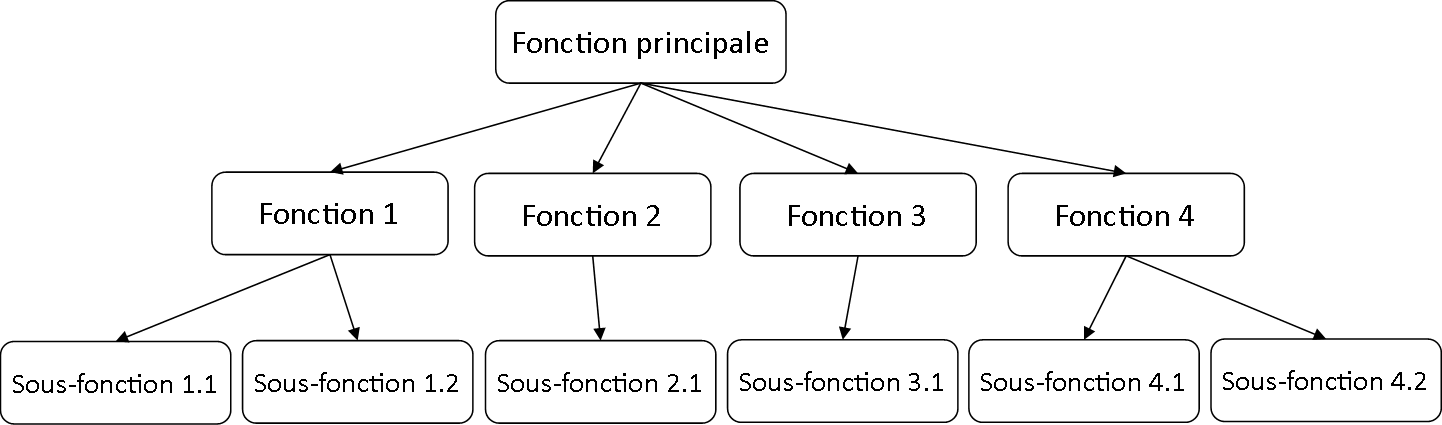
\includegraphics[width=0.75\textwidth]{img/approche_fonctionnelle.png}
	\caption{Représentation de l'approche fonctionnelle}
	\label{fig:approche_fonctionnelle}
\end{figure}


La \textbf{programmation orientés objet} est un style de programmation qui vise à identifier les structures impliquées dans un problème et à les faire interagir pour le résoudre. Elle considère un système comme un ensemble d'objets autonomes possédant des caractéristiques propres et un comportement. Ce type de programmation cherche à rassembler au même endroit les données (ou structures de données) et fonctions qui sont faites pour aller ensemble.

\begin{figure}[H]
	\center 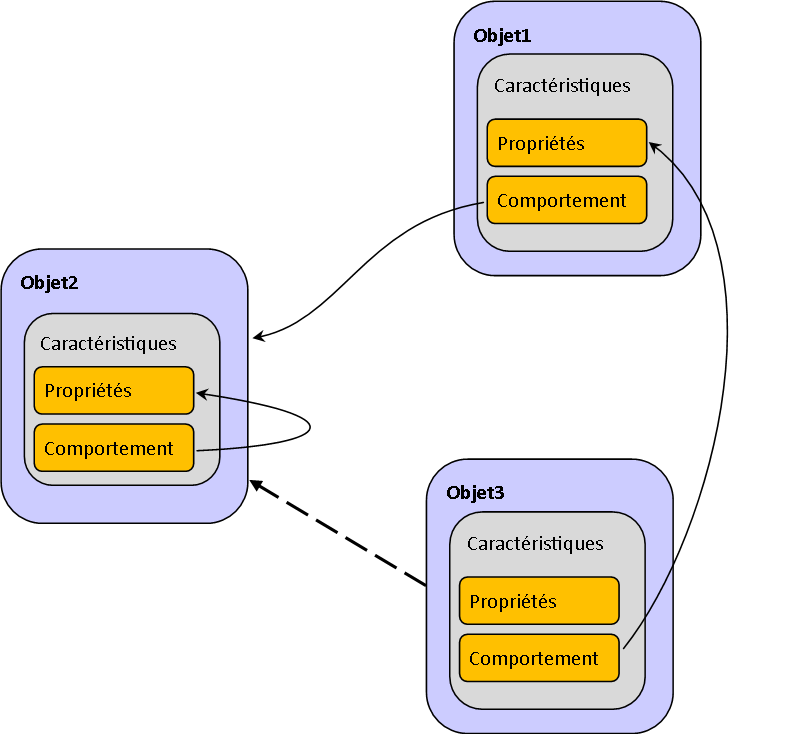
\includegraphics[width=0.5\textwidth]{img/approche_objet.png}
	\caption{Représentation de l'approche orientée objet}
	\label{fig:approche_objet}
\end{figure}

Lors des parties précédentes de ce cours, nous avons appris à utiliser des structures de données plus ou moins complexes (nombres, listes, dictionnaires, etc.). Nous avons stocké des valeurs dans ces structures, puis manipulé ces structures à l'aide d'opérateurs ou de de fonctions. En sommes, les structures manipulées possèdent des attributs (pour y stocker des valeurs) et des propriétés (les opérateurs et fonctions utilisés). Nous avons donc, sans le formaliser explicitement, manipulé des objets. Il nous reste maintenant à voir comment définir nos propres objets.


%%% ---------------------
\section{Objets, classes}
%%%
\subsection{Définitions}
Un \textbf{objet} est une entité autonome (entité du monde physique, concept, idée) décrit par une collection de propriétés et de traitements associés. L'objet est au coeur de la modélisation orientée objet.

En Python, tout est objet : une chaîne de caractères, une liste, un dictionaire, etc. Pour créer un nouvel objet, il faut dire à l'ordinateur à quoi devra ressembler cet objet. Il s'agit concrètement de choisir un modèle suivant lequel créer l'objet. En programmation orientée objet, ce modèle d'objet est appelé une \textbf{classe}.

La syntaxe Python de création d'une classe utilise le mot clé \lstinline{class} :
\begin{lstlisting}
>>> class ModeleDObjet(object):
...     pass
\end{lstlisting}

Le \lstinline{(object)} est obligatoire, nous y reviendrons ultérieurement. Ensuite, on crée l'objet à partir de ce modèle en appellant la classe :
\begin{lstlisting}
>>> mon_objet = ModeleDObjet()
\end{lstlisting}

\underline{Remarque} : par convention, on nomme les classes avec la première lettre de chaque mot en majuscule (NomDeLaClasse), et les objets avec des minuscules et des underscores (nom\_de\_l\_objet).

On dit que l'objet est une \textbf{instance} de classe. Il est possible de créer autant d'instances que l'on veut à partir d'une même classe (la fonction id(), déjà utilisée dans ce cours, retourne l'adresse mémoire d'un objet : elle permet d'identifier de manière unique un objet):
\begin{lstlisting}
>>> id(ModeleDObjet())
49253616
>>> id(ModeleDObjet())
48768592
>>> id(ModeleDObjet())
49253584
\end{lstlisting}


%%%
\subsection{Méthodes}
La classe doit donc permettre de décrire à quoi va ressembler un objet :
\begin{itemize}
	\item les attributs qui le caractérisent;
	\item les opérations qui définissent son comportement.
\end{itemize}

Les opérations qui définissent le comportement d'un objet sont appelées des \textbf{méthodes}. 
Il s'agit simplement de fonctions définies à l'intéreur de la classe. On utilise donc le mot clé \lstinline{def} :
\begin{lstlisting}
>>> class ModeleDObjet(object):
...     def une_methode(param):
...         print("Je passe dans la méthode")
...
>>> mon_objet = ModeleDObjet()
>>> mon_objet.une_methode()
Je passe dans la méthode
\end{lstlisting}

Une méthode n'existe pas en dehors de la classe :
\begin{lstlisting}
>>> une_methode()
NameError: name 'une_methode' is not defined
\end{lstlisting}

Une particularité de Python fait que, lors de l'appel d'une méthode depuis un objet, cet objet est automatiquement passé en premier paramètre de la méthode : tout se passe comme si l'interpréteur transformait l'écriture \lstinline{mon_objet.une_methode()} en \lstinline{une_methode(mon_objet)}. 

La présence de cet argument dans la définition de la méthode est obligatoire. Son absence provoque une erreur lors de l'appel de la fonction :
\begin{lstlisting}
>>> class ModeleDObjet(object):
...     def une_autre_methode():
...         print("Je passe dans l'autre méthode")
...
>>> mon_objet = ModeleDObjet()
>>> mon_objet.une_autre_methode()
TypeError: une_autre_methode() takes no arguments (1 given)
\end{lstlisting}
	
La  convention veut que l'on appelle cet argument \lstinline{self} pour faire référence à l'objet lui-même. Il s'agit d'une convention très forte en Python et ne pas la respecter risque de rendre votre programme incompréhensible pour un autre développeur.


%%%
\subsection{Attributs}
De même que pour les méthodes, qui ne sont que des fonctions attachées aux objets, les attributs sont des variables attachées aux objets. Comme pour les méthodes, ils sont accessibles en faisant précéder le nom de l'attribut du nom de l'objet :
\begin{lstlisting}
>>> mon_objet.un_attribut = 4
>>> mon_objet.un_attribut
4
>>> un_attribut		# l'attribut n'existe pas en dehors de l'objet
NameError: name 'un_attribut' is not defined
\end{lstlisting}

Deux objets peuvent avoir des valeurs d'attributs différentes :
\begin{lstlisting}
>>> mon_objet = ModeleDObjet()
>>> mon_objet.un_attribut = 4
>>> ton_objet = ModeleDObjet()
>>> ton_objet.un_attribut = "toto"
>>> mon_objet.un_attribut
4
>>> ton_objet.un_attribut
"toto"
\end{lstlisting}

Il est également possible d'accéder à un attribut depuis l'intérieur d'un objet, pour lui affecter une valeur, le modifier, l'afficher... En respectant la convention, on utilisera alors \lstinline{self} pour faire référence à l'objet lui-même :
\begin{lstlisting}
>>> class ModeleDObjet(object):
...     def affecter_attribut(self, valeur):
...         self.un_attribut = valeur
...     def modifier_attribut(self):
...         self.un_attribut += 2
...     def afficher_attribut(self):
...         print(self.un_attribut)
...
>>> mon_objet = ModeleDObjet()
>>> mon_objet.affecter_attribut(4)  # on passe la valeur 4 en paramètre de la fonction
>>> mon_objet.afficher_attribut()
4
>>> mon_objet.modifier_attribut()
>>> mon_objet.afficher_attribut
6
\end{lstlisting}


%%%
\subsection{Initialisation d'un objet}
Il est assez fréquent de vouloir créer des objets avec un état de départ contrôlé. Mettre à jour l'ensemble des attributs de tous les objets ne serait pas des plus pratiques. Aussi, afin de faciliter cette tache, Python propose une méthode spéciale pour initialiser l'état d'un objet : la méthode \lstinline{__init__()}. Lorsqu'elle est présente, cette méthode est exécutée automatiquement à la création d'un objet.
\begin{lstlisting}
>>> class ModeleDObjet(object):
...     def __init__(self):
...         self.un_attribut = "valeur initiale"
...         print("Bonjour")
...
>>> mon_objet = ModeleDObjet()
"Bonjour"
>>> mon_objet.un_attribut
"valeur initiale"
\end{lstlisting}
	
Il est possible de passer des paramètres à la méthode \lstinline{__init__()} lors de l'instanciation pour préciser certaines conditions initiales :
\begin{lstlisting}
>>> class ModeleDObjet(object):
...     def __init__(self, valeur):
...         self.un_attribut = valeur
...         print("Bonjour")
...
>>> mon_objet = ModeleDObjet("je suis vivant")
"Bonjour"
>>> mon_objet.un_attribut
"je suis vivant"
\end{lstlisting}



%%% ---------------------------------------------
\section{Principes de l'orienté objet en Python}
Faire de la programmation orientée objet suppose manipuler des classes et des objets pour résoudre les problèmes. Pour pouvoir appliquer tous les concepts de ce type de programmation, cela nécessite aussi de maîtriser trois grands principes : l'\textbf{encapsulation}, l'\textbf{héritage} et le \textbf{polymorphisme}. Nous nous attarderons dans un premier temps sur la mise en oeuvre en Python des deux principes que sont l'héritage et le polymorphisme. Puis nous aborderons en détail le concept d'encapsulation en Python.


%%%
\subsection{Héritage et polymorphisme}
L'héritage c'est la capacité de pouvoir créer une classe dérivée à partir d'une classe existante,  les attributs et méthodes de la classe existante étant automatiquement transmis à la classe dérivée. On parle également de classes mères et filles (pour respectivement classes existantes et dérivées). L'héritage est un principe qui encourage la réutilisation du code.

En Python, l'héritage est indiqué dans la signature de la classe, en remplaçant le \lstinline{object} par le nom de la classe mère :
\begin{lstlisting}
>>> class ClasseMere(object):
...     pass
...
>>> class ClasseFille(ClasseMere):  # on indique que ClasseFille hérite de ClasseMere
...     pass
...
\end{lstlisting}

Les méthodes définies dans la classe mère sont directement utilisables depuis la classe fille. Il n'y a pas besoin de les redéfinir.
\begin{lstlisting}
>>> class Bavard(object):
...     def blablabla(self):
...         print("Je ne m'arrête jamais de parler...")
...
>>> class Copieur(Bavard):
...     pass
...
>>> Copieur().blablabla()
Je ne m'arrête jamais de parler...
\end{lstlisting}

\underline{Remarque} : la syntaxe générale \lstinline{class ModeleDObjet(object)} nous indique donc que toutes les classes héritent d'une classe \lstinline{object}. Il s'agit d'un type de base en Python, au même titre que les entiers, les chaînes de caractères ou les dictionnaires.

Parfois, on souhaite hériter seulement d'une partie d'une classe, et redéfinir certaines méthodes ou attributs. Il suffira pour cela de ré-écrire la méthode dans la classe fille.
\begin{lstlisting}
>>> class Professeur(object):
...     def methode(self):
...         print("Il faut apprendre ses leçons")
...
>>> class BonEleve(Professeur): 
...     pass
...
>>> class MauvaisEleve(Professeur):
...     def methode(self):
...         print("Je n'apprend pas mes leçons")
...
>>> BonEleve().methode()
Il faut apprendre ses leçons
>>> MauvaisEleve().methode()
Je n'apprend pas mes leçons
\end{lstlisting}


Dans notre exemple précédent, BonEleve et MauvaisEleve ont les mêmes attributs et méthodes, même si elles ne font pas la même chose. On dit que les deux classes partagent une \textbf{interface} commune. La capacité à redéfinir le comportement des méthodes est le \textbf{polymorphisme}.

Avant de poursuivre, on notera que l'héritage concerne toutes les méthodes de la classe mère, y compris le constructeur (\lstinline{__init__()}) et méthodes spéciales (cf. paragraphe \ref{sec:classes_avancees}). Il est possible de redéfinir le comportement de toutes ces méthodes également.
\begin{lstlisting}
>>> class Professeur(object):
...     def methode(self):
...         print("Il faut apprendre ses leçons")
...
>>> class BonEleve(Professeur): 
...     pass
...
>>> class MauvaisEleve(Professeur):
...     def methode(self):
...         print("Je n'apprend pas mes leçons")
...
>>> BonEleve().methode()
Il faut apprendre ses leçons
>>> MauvaisEleve().methode()
Je n'apprend pas mes leçons
\end{lstlisting}

Nous avons appris à redéfinir une méthode héritée en la ré-écrivant complètement. Parfois le comportement de la classe fille ne différera que très légèrement de celui de la classe mère. Dans ce cas, il serait opportun de pouvoir récupérer le code du parent pour l'appeler dans la méthode de l'enfant en y ajoutant les précisions nécessaires. Cela est possible en Python à l'aide de la fonction \lstinline{super()} :
\begin{lstlisting}
>>> class Article(object):
...     def __init__(self, prix):
...         self.prix = prix
...
>>> class ArticleEnPromotion(Article): 
...     def __init__(self, prix, rabais):
...         self.prix = super(ArticleEnPromotion, self).__init__(prix) * rabais
...
>>> Article(10).prix
10
>>> ArticleEnPromotion(10, 0.8).prix
8
\end{lstlisting}


%%%
\subsection{Classe abstraite}
Une classe abstraite est une classe qui ne peut pas être instanciée. Une telle classe est utile uniquement pour définir par héritage d'autres classes.

Il n'est pas possible, en raison du typage dynamique en Python, de définir réellement une classe abstraite. Certaines astuces consistant à lever une exception dans le constructeur de la classe abstraite permettent de s'affranchir de cette limitation du langage. 



%%%
\subsection{Héritage multiple}
Il arrive parfois que l'on veuille construire une classe en réutilisant les attributs et méthodes définies dans plusieurs autres classes. Il s'agit d'un \textbf{héritage multiple} : une classe fille hérite de plusieurs classes mères. Il faut dans ce cas appeler explicitement le constructeur des classes mères.
\begin{lstlisting}
>>> class Carre(object):
...     __init__(self, cote):
...         self.cote = cote
>>> class Couleur(object): 
...     __init__(self, r, v, b):
...         self.rvb = (r, v, b)
>>> class CarreColore(Carre, Couleur):
...     def __init__(self, cote, r, v, b):
...         Carre.__init__(self, cote)
...         Couleur.__init__(self, r, v, b)
...
>>> CarreColore(4, 255, 0, 0).rvb
(255, 0, 0)
>>> CarreColore(4, 255, 0, 0).cote
4
\end{lstlisting}


%%%
\subsection{Encapsulation}
L'encapsulation est le fait de rassembler les données et méthodes au sein d'une structure en cachant les détails de l'implémentation. Ce concept permet de modifier les méthodes ou d'ajouter des attributs sans avoir à redéfinir complètement les objets.

Contrairement à d'autres langages comme le Java ou le C++, la structure du langage Python ne force pas l'encapsulation des données. Par défaut, il est toujours possible d'avoir accès aux attributs et méthodes d'une classe, même depuis l'extérieur de celle-ci (c'est ce que nous avons fait depuis le début de ce chapitre). En revanche, les programmeurs Python ont adopté un consensus sur l'accès aux attributs qui consiste :
\begin{itemize}
	\item à préfixer d'un \_ les attributs privés : \lstinline{_mon_attribut_prive}
	\item à écrire normalement les attributs publics : \lstinline{mon_attribut_public}
\end{itemize}


Utiliser un attribut privé ne signifie pas qu'il ne sera jamais possible d'y accéder depuis l'extérieur de l'objet. Lorsque cela sera nécessaire le développeur utilisera des \textbf{accesseurs} et \textbf{mutateurs}. Ces noms désignent juste des fonctions qui permettrons respectivement de lire et modifier la valeur de l'attribut d'un objet. Naturellement, en fonction des besoins, on écrira l'une ou l'autre (ou les deux ou aucune) de ces deux fonctions.

Pour écrire un accesseur ou un mutateur, on utilise des \textbf{décorateurs} de fonction. Un décorateur est une inscription que l'on place juste avant la signature de la fonction et qui permet de préciser l'utilisation de la fonction. Ils prennent la forme suivante :
\begin{lstlisting}
@decorateur
def ma_fonction(args):
	instructions
\end{lstlisting}

Pour créer un accesseur, le décorateur sera \lstinline{@property}. Cela transforme la méthode en propriété. Il n'est alors plus nécessaire d'utiliser les parenthèses pour appeler la méthode.
\begin{lstlisting}
>>> class Carre(object):
...     def __init__(self, cote):
...         self._cote = cote
...
...     @property
...     def cote(self):
...         return self._cote
...
>>> Carre(4).cote
4
\end{lstlisting}

On utilisera également le décorateur \lstinline{@property} lorsque l'on souhaitera créer des attributs dérivés.
\begin{lstlisting}
>>> class Carre(object):
...     def __init__(self, cote):
...         self._cote = cote
...
...     @property
...     def surface(self):
...         return self._cote ** 2
...
>>> Carre(4).surface
16
\end{lstlisting}

Pour un mutateur, il prendra la valeur \lstinline{@nom.setter} où nom est le nom de l'attribut (celui visible depuis l'extérieur, donc le nom de la propriété définit grâce à l'accesseur). 
\begin{lstlisting}
>>> class Carre(object):
...     def __init__(self, cote):
...         self._cote = cote
...
...     @property
...     def cote(self):
...         return self._cote
...
...     @cote.setter
...     def cote(self, valeur):
...         self._cote = valeur
...
>>> mon_carre = Carre(4)
>>> mon_carre.cote
4
>>> mon_carre.cote = 2
>>> mon_carre.cote
2
\end{lstlisting}

Nous utiliserons également un dernier décorateur nous permettra de supprimer un attribut : \lstinline{@nom.deleter}.

L'utilisation d'accesseurs et mutateurs (on parle aussi de getter / setter), au delà de respecter la convention ayant cours dans le milieu des développeurs Python, nous permet de contrôler le type et éventuellement d'effectuer des opérations sur les valeurs affectées dans les attributs. En effet le typage dynamique fort en Python ne nous permet pas de verrouiller le type d'un attribut.

Voici un exemple complet :
\begin{lstlisting}
>>> class Personne(object):
...     def __init__(self, nom):
...         self._nom = nom
...
...     @property
...     def nom(self):
...         return self._nom
...
...     @nom.setter
...     def nom(self, valeur):
...         if not isinstance(valeur, str):
...             raise ValueError("La valeur attendue pour le nom doit être un string")
...         self._nom = valeur.capitalize()
...
...     @nom.deleter
...     def nom(self):
...         del(self._nom)
...
>>> toto = Personne("Papa")
>>> toto.nom
Papa
>>> toto.nom = 45
ValueError: La valeur attendue pour le nom doit être un string
>>> toto.nom = "maman"
>>> toto.nom		 
Maman     # remarquez la majuscule automatique sur la 1ère lettre
>>> del(toto.nom)
>>> toto.nom
AttributeError: 'Personne' object has no attribute '_nom'
\end{lstlisting}



%%% -------------------
\section{Concepts avancés avec les classes}
\label{sec:classes_avancees}

%%%
\subsection{Méthodes spéciales}
On appelle \textbf{méthode spéciale} une méthode qui est exécutée automatiquement lorsque des conditions particulières sont observées. C'était par exemple le cas du constructeur de l'objet \lstinline{__init__()} qui est lancé automatiquement à la création d'un objet. Les méthodes spéciales sont préfixés et suffixés avec deux underscores.

Nous présentons ici quelques unes des méthodes que nous pouvons rencontrer :
\begin{itemize}
	\item la méthode \lstinline{__str__()} : elle est déclanchée lorsque la commande \lstinline{print} est appelée sur un objet. Elle permet de personnaliser ce qui est affiché.

	\begin{lstlisting}
>>> class ModeleDObjetStandard(object):
...     pass
>>> print(ModeleDObjet())
<__main__.ModeleDObjetStandard object at 0x059F0190>
>>> class ModeleDObjetPersonnalise(object):
...     def __str__(self):
...         return "Objet personnalisé (identifiant {})".format(id(self))
>>> print(ModeleDObjetPersonnalise())
Objet personnalisé (identifiant 6912457)
	\end{lstlisting}
	
	\item la méthode \lstinline{__repr__()} est appelée lorsque l'on tape directement le nom d'un objet. Elle permet de remplacer l'affichage par défaut qui n'est pas très parlant (du type \lstinline{<__main__.ModeleDObjet object at 0x0342C390>}). Elle est aussi appelé lorsque l'on affiche une liste.
	
	\item méthodes de comparaison : \lstinline{__eq__()}, \lstinline{__lt__()}, \lstinline{__le__()},\lstinline{__gt__()}, \lstinline{__ge__()}, \lstinline{__ne__()} pour respectivement $=$, $<$, $<=$, $>$, $>=$ et $!=$
	
	Dans l'exemple suivant, on définit une classe Etudiant avec deux attributs : une note en informatique et une note en géodésie. On utilise ensuite la méthode \lstinline{__le__()} permettant de comparer les étudiants : un étudiant est supérieur à un autre s'il possède une meilleure note en informatique).
	\begin{lstlisting}
>>> class Etudiant(object):
...     def __init__(self, informatique, geodesie):
...         self.note_info = informatique
...         self.note_geodes = geodesie
...
...     def __le__(self, other):
...         if self.note_info > other.note_info:
...             return True
...         else:
...             return False
>>> albert = Etudiant(15, 0)
>>> alfred = Edutiant(12, 20)
>>> albert > alfred
True
	\end{lstlisting}
	
	\item les opérateur mathématiques ($+$, $-$, $*$, $**$, etc.) sont également couvert par des méthodes spéciales : \lstinline{__add__()}, \lstinline{__sub__()}, \lstinline{__mul__()}, \lstinline{__truediv__()}, etc. (cf.table \ref{tab:methodes_speciales_operateurs}).
	
	\begin{table}[H]
	\begin{center}
		\begin{tabular}{|c|c|}
			\hline
			\textbf{Opérateur} & \textbf{Méthode} \\
			\hline
			\lstinline{+} & \lstinline{__add__} \\
			\lstinline{-} & \lstinline{__sub__}\\
			\lstinline{*} & \lstinline{__mul__} \\
			\lstinline{**} & \lstinline{__pow__} \\
			\lstinline{/} & \lstinline{__div__} \\
			\lstinline{//} & \lstinline{__truediv__} \\
			\lstinline{%} & Reste d'une division entière (modulo) \\
			\hline
		\end{tabular}
		\caption{Méthodes spéciales pour surcharger les opérateurs}
		\label{tab:methodes_speciales_operateurs}
	\end{center}
\end{table}

	\item les méthodes \lstinline{__getitem__()}, \lstinline{__setitem__()} et \lstinline{__delitem__()} qui permettent de définir ce que l'on obtiendra lorsque l'on écrira respectivement \lstinline{object[i]}, \lstinline{object[i] = valeur} et \lstinline{del object[i]}.
	
	\item les méthodes \lstinline{__float__()}, \lstinline{__int__()}, \lstinline{__str__()} pour convertir un objet dans un format donné.
	
	\item la méthode \lstinline{__len__()} est appelée lorsque l'on souhaite connaître la taille d'un objet avec la méthode \lstinline{len(objet)}.

	\item ...
\end{itemize}

Les méthodes spéciales couvrent ainsi la grande majorité des opérations classiques que l'on est amené à effectuer sur les objets en Python.

 
%%%
\subsection{Attributs et méthodes de classe}
Un \textbf{attribut de classe} est un attribut qui appartient à la classe et non plus à l'objet. Sa valeur est partagée par toute les instances de la classe.

\begin{lstlisting}
class ModeleDObjet:
    attribut_de_classe = 'meme valeur pour tous les objets'

    def __init__(self):
		    self.attribut_d_objet = "valable seulement pour l'objet en cours"
\end{lstlisting}

Il n'est pas nécessaire de créer une instance de classe pour avoir accès à l'attribut de classe.
\begin{lstlisting}
>>> print(ModeleDObjet.attribut_de_classe)
meme valeur pour tous les objets
>>> print(ModeleDObjet.attribut_d_objet)
AttributeError: type object 'ModeleDObjet' has no attribute 'attribut_d_objet'
\end{lstlisting}

En revanche, une instance de la classe à bien accès aux deux attributs :
\begin{lstlisting}
>>> print(ModeleDObjet().attribut_de_classe)
meme valeur pour pour tous les objets
>>> print(ModeleDObjet().attribut_d_objet)
valable seulement pour l'objet en cours
\end{lstlisting}

Sur le même principe, on peut créer des \textbf{méthodes de classe}. On utilise pour cela un décorateur de fonction : \lstinline{@classmethod}. La convention dans ce cas est d'utiliser \lstinline{cls} à la place de \lstinline{self}. En effet, avec une méthode de classe c'est la classe elle-même qui est passée en premier paramètre de la fonction et non plus l'objet courant.
\begin{lstlisting}
class ModeleDObjet:
    
    @classmethod
    def methode_de_classe(cls):
		    print("Je suis une méthode de classe")
\end{lstlisting}

L'intérêt des méthodes et attributs de classes et de regrouper au même endroit les choses qui traitent de la même chose. Leur usage permet généralement d'éviter le recours à des attributs globaux dont le comportement n'est pas toujours maîtrisable.


%%%
\subsection{Les gestionnaires de contexte}
Les \textbf{gestionnaires de contexte} sont des objets qui nous permettent d'employer une syntaxe du type \lstinline{with objet as alias:}. Sans en donner le nom, nous en avons déjà utilisé, par exemple pour manipuler un fichier (cf. paragraphe \ref{sec:fichiers}).

Une manière de créer un gestionnaire de contexte en Python est de définir une classe possédant deux méthodes spéciales : \lstinline{__enter__} et \lstinline{__exit__}. La fonction \lstinline{__enter__} est déclenchée à l'entrée dans le bloc et permet de définir ce qui sera récupéré par le mot clé \lstinline{as}, tandis que la fonction \lstinline{__exit__} est déclenchée à la sortie du bloc \lstinline{with}.

Dans l'exemple suivant, on définit un gestionnaire de contexte qui sert uniquement à afficher un temps d'exécution : le temps est enregistré à l'entrée dans le bloc et à la sortie, où on affiche alors la différence :
\begin{lstlisting}
import time
class Compteur(object):
    def __init__(self, nom):
        self.nom = nom
    def __enter__(self):
        self.t_debut = time.time()
    def __exit__(self, exc_ty, exc_val, exc_tb):
        t_fin = time.time()
        print('{}: {}'.format(self.nom, t_fin - self.t_debut))
\end{lstlisting}

On peut l'utiliser pour mesurer le temps d'exécution de n'importe quel bloc d'instructions. Par exemple, pour comparer les performances de boucles \lstinline{while} et \lstinline{for} :
\begin{lstlisting}
>>> n = 1000000
>>> with Compteur('Boucle for'):
...     for i in range(n):
...         pass
...
Boucle for: 0.42704200744628906
>>> with Compteur('Boucle while'):
...     while n > 0:
...         n -= 1
...
Boucle while: 1.0651071071624756
\end{lstlisting}


%%%---------------
%%% Les exceptions
%%%---------------
\newpage
\part{Les exceptions}
\chapter{}

%%% ------------------------------------
\section{Généralités}
Réaliser certaines opérations est parfois impossible, comme par exemple diviser par zéro. Python fournit un mécanisme pour gérer ce genre d'erreurs survenues lors de l'exécution d'un programme : les \textbf{exceptions}.

Le traitement des exceptions permet d'apporter des solutions à des situations qui auraient entraîné une interruption du programme. Il se découpe en trois étapes :
\begin{enumerate}
	\item détection de l'erreur, réalisation d'une condition exceptionnelle;
	\item interruption du déroulement normal et lancement d'une exception;
	\item traitement de l'erreur dans le contexte courant et/ou propagation de cette erreur vers un niveau supérieur.
\end{enumerate}

Les exceptions fournissent une moyen efficace de répondre à un événement inhabituel qui est en train de se produire (erreur, cas particulier, événement inattendu, etc.). En effet, une exception ne fait pas qu'interrompre le cours normal d'un programme, elle apporte également des informations sur la source de l'erreur. 

A ce stade du cours, vous avez certainement déjà rencontré des exceptions. Elles déclenchent l'affichage dans la console d'un message ressemblant à celui-ci :
\begin{lstlisting}
Traceback (most recent call last):
  File "<pyshell#1>", line 1, in <module>
    import et-patatras
ImportError: No module named 'et-patatras'
\end{lstlisting}

On y retrouve toujours deux éléments importants :
\begin{itemize}
	\item sur la dernière ligne, le \textit{type de l'exception} ainsi que la description la cause de l'erreur;
	\item au dessus, un à plusieurs blocs de trois lignes, appelé la \textit{stack trace}, et qui indique les différents appels ayant conduit à l'erreur.
\end{itemize}

Une erreur se lit donc de bas en haut : le type de l'exception, l'instruction qui a causé l'erreur, et la pile d'appels permettant de retrouver l'origine de l'erreur.

Le type de l'exception se réfère à des catégories bien précises. Les exceptions sont des classes qui dérivent toutes d'une classe mère \lstinline{BaseException}. La hiérarchie des exceptions les plus fréquemment rencontrées est présentée ci-dessous :

\fbox{
	\begin{footnotesize}
		\begin{minipage}{0.9\textwidth}
			BaseException : regroupe l'ensemble des exceptions
			\begin{itemize}
				\item SystemExit : arrêt du programme
				\item KeyboardInterupt : l'utilisateur appuie sur des touches interruption du programme
				\item Exception : regroupe les exceptions qui ne se rapportent pas à la fermeture du programme
				\begin{itemize}
					\item StopIteration : survient lorsque la fonction next d'un itérateur ne retourne plus rien
					\item ArithmeticError : classe mère des exceptions sur les opérations mathématiques
					\begin{itemize}
						\item OverflowError : résultat d'une expression trop grand pour être représenté
						\item ZeroDivisionError : division par zéro
					\end{itemize}
					\item AssertionError : échec d'une instruction assert
					\item AttributeError : utilisation d'un attribut inexistant d'un objet
					\item EOFError : 
					\item ImportError : import d'un module inexistant
					\item LookupError : classe mère des exceptions sur les index ou clés
					\begin{itemize}
						\item IndexError : accès à un élément d'une séquence avec un indice qui n'existe pas 
						\item KeyError : accès à un élément d'un dictionnaire avec une clé qui n'existe pas
					\end{itemize}
					\item NameError : la variable ou fonction manipulée n'est pas déclarée
					\item OSError : classe mère pour toutes les erreurs de manipulation de fichier
					\begin{itemize}
						\item ConnectionError : 
						\item FileNotFoundError : le fichier n'existe pas
						\item PermissionError : pas les droit pour effectuer l'opération sur un fichier
					\end{itemize}
					\item ReferenceError
					\item RuntimeError
					\begin{itemize}
						\item NotImplementedError
					\end{itemize}
					\item SyntaxError : erreur de syntaxe générale
					\begin{itemize}
						\item IndentationError : erreur d'indentation
					\end{itemize}
					\item SystemError
					\item TypeError : le type de la variable ne permet pas d'effectuer l'opération demandée
					\item ValueError : le type est correct, mais pas la valeur
				\end{itemize}
			\end{itemize}
		\end{minipage}
	\end{footnotesize}
}

On notera que les exceptions sont, comme toutes choses en Python, des objets. Il est donc possible de définir ses propres types d'exception pour gérer des erreurs spécifiques à un programme. On créera pour cela des classes héritant de \lstinline{BaseException} ou d'une exception qui en dérive.


%%% --------------------------------
\section{Traitement d'une exception}
Lorsqu'une exception est activée, on dit qu'elle est levée. Pour \textbf{lever une exception} soit même, on utilise la syntaxe suivante :
\begin{lstlisting}
raise NomDeLExceptionALever("Message d'explication")
\end{lstlisting}

Une exception peut être levée lorsque l'on est dans une configuration que l'on sait non prévue par le programme. Par exemple le type d'un paramètre n'est pas celui attendu :
\begin{lstlisting}
def ma_fonction(param):
    if not isinstance(param, int):
			raise TypeError("Le paramètre doit être un entier")
raise NomDeLExceptionALever("Message d'explication")
\end{lstlisting}

Si le paramètre n'est pas un entier, une exception est soulevée :
\begin{lstlisting}
>>> ma_fonction(1.5)
Traceback (most recent call last):
  File "<pyshell#38>", line 1, in <module>
    ma_fonction(1.5)
  File "<pyshell#36>", line 2, in ma_fonction
    if not isinstance(param, int):raise TypeError("Le paramètre doit être un entier")
TypeError: Le paramètre doit être un entier
\end{lstlisting}

Mais l'intérêt des exceptions ne se limite pas à arrêter le programme en affichant de jolis messages d'erreurs. Elles permettent avant tout de gérer des cas particuliers pour justement éviter que le programme ne fasse que s'arrêter. Lorsqu'un bloc de code est susceptible de soulever une exception, on utilise des instructions \lstinline{try/except} :
\begin{lstlisting}
try:
    instructions succeptibles de soulever une exception
except NomDeLException:
    instructions à exécuter si l'exception est levée
\end{lstlisting}

Par exemple :
\begin{lstlisting}
try:
    return 1 / x
except ZeroDivisionError:
    return float('inf')
\end{lstlisting}

Si x vaut 0, Python va lever une exception \lstinline{ZeroDivisionError}, le bloc \lstinline{except} sera appelé et la valeur \lstinline{float('inf')} sera retournée.

Cela suppose de savoir quelle exception on souhaite intercepter (en cas de doute, le plus simple est généralement de provoquer volontairement l'exception).

Il est possible de gérer plusieurs types d'exceptions pour le même bout de code.
\begin{lstlisting}
liste = ['poule', 'vache', 'cochon']
try:
    return liste[10 % i]
except ZeroDivisionError, IndexError:
    return None
except TypeError:
    print("i doit être un nombre")
\end{lstlisting}

\underline{Remarque} : il est aussi possible de ne pas spécifier le type d'exception à attraper, pour que Python intercepte toutes les erreurs possibles.
\begin{lstlisting}
liste = ['poule', 'vache', 'cochon']
try:
    return liste[10 % i]
except:
    print("Problème...")
\end{lstlisting}

C'est généralement une mauvaise idée, car si une erreur arrive, on sera incapable de savoir ce qui l'a causée.

La structure \lstinline{try/else} peut être complétée par des clauses \lstinline{else} et/ou \lstinline{finally}.

La clause \lstinline{else} s'exécute lorsqu'aucune erreur n'a été interceptée à l'exécution du bloc de code \lstinline{try}. La clause \lstinline{finally} permet d'exécuter des instructions dans tous les cas, qu'une exception ai été levée ou pas. Elle est parcourue après toutes les autres clauses.

Exemple avec l'ouverture d'un fichier 
\begin{lstlisting}
chemin = "D:\..."
try:
    fichier = open(chemin, 'r')  # tentative d'ouverture du fichier
except FileNotFoundError:
    print("Le fichier n'existe pas")
except IOError:
    print("Erreur à la lecture du fichier")
else:
    print("Fichier ouvert")
		print(fichier.read())  # affichage du contenu
finally:
    fichier.close()  # on referme le fichier
\end{lstlisting}


% mot clé assert




%%%--------
%%% Annexes
%%%--------
\newpage
\part{Annexes}
\chapter{}

\section*{Installer des librairies Python}
\label{sec:install_paquets_python}
Une des grandes forces de Python, c'est la multitude de libraires disponibles. On est donc souvent amené à installer de nouvelles librairies (on par le aussi de paquets). Pour installer un paquet Python, la première méthode est de télécharger les sources, qui contiennent un fichier \lstinline{setup.py}, puis de saisir dans une invite de commande :
\begin{lstlisting}
python setup.py install
\end{lstlisting}

Ce n'est pas des plus pratique, notamment l'étape du téléchargement (où trouver le paquet? comment savoir si c'est bien la dernière version?). De plus, il arrive fréquemment que des paquets nécessitent la présence d'autres paquets pour pouvoir fonctionner (on parle de dépendances). On doit donc trouver tous les paquets, puis les télécharger et installer individuellement...

Python nous facilite la vie avec un système de gestion de paquets : \textbf{pip}. Depuis les dernières version de Python, pip est installé par défaut. pip permet d'installer simplement un paquet en saisissant\footnote{Selon la configuration du poste, il peut être nécessaire de se placer dans le répertoire Script de l'installation de Python.} :
\begin{lstlisting}
pip install paquet
\end{lstlisting}

La syntaxe n'apporte pas grand chose, mais...
\begin{itemize}
	\item il n'est plus nécessaire de télécharger le paquet : pip s'en charge tout seul
	\item il n'est plus nécessaire de récupérer les dépendances : pip s'en charge tout seul
\end{itemize}

En arrière plan, pip se connecte au site \url{http://pypi.python.org/pypi} où chaque développeur Python est libre d'enregistrer ses paquets, en respectant quelques conditions, dont le renseignement de dépendances.

pip permet de choisir la version que l'on souhaite installer. Par exemple, la version 1.8 de Django :
\begin{lstlisting}
pip install Django==1.8
\end{lstlisting}

Il est également possible de mettre à jour un paquet :
\begin{lstlisting}
pip install Django --upgrade
\end{lstlisting}

Mais également de désinstaller les paquets devenus inutiles :
\begin{lstlisting}
pip uninstall Django
\end{lstlisting}
	
Bref, la méthode pip ne présente que des avantages. Elle atteindra ses limites lorsque l'on cherchera à installer de grosses librairies types PyQt ou avec des extensions en C type numpy.

\vspace{2em}

Lorsque l'on commence à beaucoup développer, il arrive que l'on soit amené à travailler sur des projet basées sur des versions différentes d'une même librairie. Parfois on souhaite aussi juste tester une librairie ou une version sans modifier tous notre environnement. \textbf{virtualenv} est la solution à ce genre de problèmes.

Il s'agit d'un paquet Python qui permet de créer des espaces de travail Python isolés les uns des autres. Pour l'installer, on fait :
\begin{lstlisting}
pip install virtualenv
\end{lstlisting}

On crée ensuite un environnement virtuel avec la commande :
\begin{lstlisting}
virtualenv /chemin/de/l/espace/de/travail
\end{lstlisting}

Pour travailler dans cet environnement virtuel, on lance le fichier activate.bat contenu dans le répertoire. Une fois dans l'environnement virtuel, on peut installer nos paquets Python avec classiquement avec pip. Ils ne seront visibles que depuis l'environnement virtuel.



%\section{L'encodage en Python}
%encodage utf-8


%\section{Python 2 vs. Python 3}
%différences principales entre python 2 et python 3
%quelle version je dois utiliser ?


\section*{Choix d'une implémentation de Python}
En introduction de ce cours (chapitre 1.5. Exécution d'un programme en Python), nous avons définit l'interpréteur Python comme un programme exécutant des programmes écrit en Python. Nous avons également précisé que cet interpréteur est lui-même écrit dans un langage différent de Python, mais sans donner plus de détail sur ce langage. En réalité, il existe plusieurs interpréteurs Python répondant à différentes problématiques et écrits dans différents langages.

\textbf{CPython} est l'interpréteur par défaut. C'est le standard d'implémentation, celui qui est utilisé par une majorité de personnes. L'interpréteur Python est écrit en C. Il est performant pour l'utilisation d'outils en C depuis Python.

Pour rendre performante l'utilisation d'outils Java ou .Net avec Python, d'autres implémentation de Python ont été développées : respectivement Jython\footnote{\url{http://www.jython.org/}} et IronPython\footnote{\url{http://ironpython.net/}}. Le bytecode produit par ces interpréteur n'est pas compatible avec celui d'une machine CPython.

\textbf{Stackless}\footnote{\url{http://www.stackless.com}} est une autre implémentation de Python conçue pour une utilisation très ciblée : l'amélioration des performances lors des traitements multi-tâches.

\textbf{PyPy}\footnote{\url{http://pypy.org/}} est une mise en oeuvre du langage Python qui présente la particularité d'être écrite en elle-même en Python. L'objectif de PyPy est d'aboutir à une version plus rapide que l'implémentation en C classique. Les porteurs du projet rapportent des gains de performance compris entre *5 et *100. Ils estiment également que leur interpréteur n'est pas encore assez stable pour être déployée massivement.

\textbf{Cython}\footnote{\url{http://cython.org/}} permet de transformer du Python en C, afin de l'embarquer dans un autre code C, et inversement de permettre des appels de C en Python plus faciles. Cet interpréteur écrit en C permet ainsi de compiler un programme autonome écrit en Python.

D'autres implémentation du langage Python existent pour répondre à d'autres besoins spécifiques. Le développeur n'aura pratiquement jamais à se poser la question de l'implémentation de Python à choisir pour un projet. Elles sont à considérer comme des bonus qui peuvent aider un développeur chevronné à résoudre un problème particulier.



%%%--------------
%%% Bibliographie
%%%--------------
\newpage
\section*{Bibliographie}

Un peu de lecture pour en apprendre plus sur le langage Python :

\vspace{2cm}

Downez Allen, \textit{Think Python (How to think like a computer scientist)}, 2012, Green Tea Press

Bersini Hugues, \textit{La programmation orientée objet}, 2013, Eyrolles

Beazley David and Jones Brian, \textit{Python Cookbook 3rd edition}, 2013, O'Reilly

Lambert Kenneth A., \textit{Fundamentals of Python}, 2010, Cengage Learning

Lutz Mark, \textit{Programming Python 4th edition}, 2010,	O'Reilly

Lutz Mark, \textit{Learning Python 5th edition}, 2013,O'Reilly

Romano Fabrizio, \textit{Learning Python}, 2015, Packt Publishing

Dupré Xavier, \textit{Programmation avec le langage Python}, 2010, ENSAE, \url{http://www.xavierdupre.fr/enseignement/initiation/initiation_via_python_ellipse_mai_2010.pdf}

Swinnen Gérard, \textit{Apprendre à programmer avec Python 3}, 2012, \url{http://inforef.be/swi/download/apprendre_python3_5.pdf}

Site Sam\&Max : \url{http://sametmax.com/cours-et-tutos/}


%\part{Index}
%\chapter{}


\end{document}